% % Preamble BEGINN %%%%%%%%%%%%%%%%%%%%%%%%%%%%%%%%%%%%%%%%%%%%%%%%%%%%%%%%%

%%% Preamble (Dokumentenklasse)
% ------------------------------------------------------------------------
% LaTeX - Preambel ******************************************************
% ------------------------------------------------------------------------
% Dokumentklasse (Koma Script)
% ------------------------------------------------------------------------
% basiernd auf www.matthiaspospiech.de/latex/vorlagen Diplomarbeit kompakt
% ========================================================================
\documentclass[%
   %draft,            % Entwurfsstadium
   final,             % fertiges Dokument
   12pt,              % Schriftgroesse der Grundschrift
   bigheadings,       % gro�e �berschriften
   ngerman,           % wird an andere Pakete weitergereicht
   a4paper,           % Papierformat
   BCOR5mm,          % Bindekorrektur: Zus�tzlicher Rand auf der Innenseite
   DIV14,            % Seitengr��e (siehe Koma Skript Dokumentation !)
   1.1headlines,     % Zeilenanzahl der Kopfzeilen
   pagesize,         % Schreibt die Papiergroesse in die Datei.
   oneside,          % Einseitiges Layout
%   twoside,          % Zweiseitiges Layout
   openright,        % Kapitel beginnen immer auf der rechten Seite
   titlepage,        % Titel als einzelne Seite ('titlepage' Umgebung)  
   headsepline,      % Linie unter Kolumnentitel ()
   footsepline,		 % Linie �ber Seitenzahl
%   plainheadsepline, % Linie unter Kolumnentitel () plain Seitenstil
   nochapterprefix,  % keine Ausgabe von 'Kapitel:'
   bibtotoc,         % Bibliographie ins TOC
%	bibtotocnumbered, % Bibliographie ins TOC mit Kapitelnummer
   tocindent,        % eingereuckte Gliederung
   listsindent,      % eingereuckte LOT, LOF
   pointlessnumbers, % �berschriftnummerierung ohne Punkt, siehe DUDEN !
   cleardoubleempty, % Leere linke Seite bei Zweiseitenlayout vor Kapitel
   fleqn,            % Formeln werden linksbuendig angezeigt
%   parindent,        % Absatz mit Einzug (Standard)
   halfparskip,      % Absatz halbe Zeile Abstand
%   parskip,          % Absatz ganze Zeile Abstand
]{scrbook}%     Klassen: scrartcl, scrreprt, scrbook


%%% Alle Namen usw. im Titel und im hyperref-Paket
% ------------------------------------------------------------------------
% LaTeX - Preambel ******************************************************
% ------------------------------------------------------------------------
% pre-work
% ========================================================================
% % ToDo kennzeichnen
\newcommand{\workTodo}[1]{\textcolor{red}{todo: #1}}

% % F�r Datum und Zeit in Fusszeile
% % !!!Inhalt bei Fertigstellung der Arbeit l�schen
\newcommand{\workMarkDateTime}{\workTodo{\today{} - \thistime\ Uhr}}

% % Alle Namen werden im Titel und im hyperref-Paket eingetragen
% % !!! Ueberall f�r <Wert> das Entsprechende eintragen

 % <Typ> Studienarbeit, Dipolmarbeit, Studienarbeit oder Bachlor-Abschlussarbeit
\newcommand{\workTyp}{Assignment\xspace}

 % <Titel> der Arbeit
\newcommand{\workTitel}{PCM}

 % <Studiengang> z.B. Kommunikationstechnik
\newcommand{\workStudiengang}{Technische Informatik\xspace}

% <Semester> mit Jahr z.B. Sommersemester 2008  
\newcommand{\workSemester}{Sommersemester 2017\xspace}

% <Name> des Studenten
\newcommand{\workNameStudent}{Antonio Parrotta\xspace}

% <Pruefer> Name des pr�fenden (betreuenden) Professor an der Hochschule
\newcommand{\workPruefer}{Dr. x\xspace} 


% %%% Nur bei Abschluss-Arbeiten

% <Datum> der Abgabe der Arbeit (Eidesstatliche Erkl�rung)
\newcommand{\workDatum}{\today\xspace}

% <Zweitpr�fer>
\newcommand{\workZweitPruefer}{Dipl.-Ing. xy \xspace}

% %%% Nur bei Industrie-Arbeiten:

% <Firma>
\newcommand{\workFirma}{IT-Designers GmbH\xspace}

% Firmenlogo Name hier anpassen, Gr��e (wenn m�glich) nicht �ndern
%\newcommand{\workFirmenLogo}{\includegraphics[width=5cm]{fig/aa-titel/Bosch_4C_S}} 


%%% Preamble (Pakete)
% ------------------------------------------------------------------------
% LaTeX - Preambel ******************************************************
% ------------------------------------------------------------------------
% Packages
% ------------------------------------------------------------------------
% basiernd auf www.matthiaspospiech.de/latex/vorlagen Diplomarbeit kompakt
% ========================================================================

% Inhalt:
% 1. Einige Pakete muessen unbedingt vor allen anderen geladen werden
% 2. Fonts Fonts Fonts
% 3. Math Packages
% 4. Symbole
% 5. text related packages
% 6. Pakete zum Zitieren
% 7. PDF related packages
% 8. Tables (Tabular)
% 9. figures and placement
% 10. verbatim packages
% 11. science packages
% 12. layout packages

% ~~~~~~~~~~~~~~~~~~~~~~~~~~~~~~~~~~~~~~~~~~~~~~~~~~~~~~~~~~~~~~~~~~~~~~~~
% Encoding der Dateien (sonst funktionieren Umlaute nicht)
% Empfohlen latin1, da einige Pakete mit utf8 Zeichen nicht
% funktionieren, z.B: listings, soul.

\usepackage[latin1]{inputenx} % ISO-8859-1
%\usepackage[ansinew]{inputenx} % Windows-Standard (CP1252) (baut auf ISO 8859-1 und ISO 8859-15 auf)
%\usepackage[utf8]{inputenc}

% ~~~~~~~~~~~~~~~~~~~~~~~~~~~~~~~~~~~~~~~~~~~~~~~~~~~~~~~~~~~~~~~~~~~~~~~~
% 1. Einige Pakete muessen unbedingt vor allen anderen geladen werden
% ~~~~~~~~~~~~~~~~~~~~~~~~~~~~~~~~~~~~~~~~~~~~~~~~~~~~~~~~~~~~~~~~~~~~~~~~
%
\usepackage{xspace} % Define commands that don't eat spaces.
\usepackage{ifpdf} % Fuer Pakete/Paketoptionen, die nur fuer pdf benoetigt werden \ifpdf \else \fi
\usepackage{calc} % Calculation with LaTeX
\usepackage[english, ngerman]{babel} % Languagesetting
\usepackage[table]{xcolor} % Farben
\usepackage[]{graphicx} % Bilder
\usepackage{subfig}
%\usepackage{epstopdf} % If an eps image is detected, epstopdf is automatically called to convert it to pdf format.
\usepackage[]{amsmath} % Amsmath - Mathematik Basispaket
\usepackage{ragged2e} % Besserer Flatternsatz (Linksbuendig, statt Blocksatz)

% ~~~~~~~~~~~~~~~~~~~~~~~~~~~~~~~~~~~~~~~~~~~~~~~~~~~~~~~~~~~~~~~~~~~~~~~~
% 2. Fonts Fonts Fonts
% ~~~~~~~~~~~~~~~~~~~~~~~~~~~~~~~~~~~~~~~~~~~~~~~~~~~~~~~~~~~~~~~~~~~~~~~~

\usepackage[T1]{fontenc} % T1 Schrift Encoding (notwendig f�r die meisten Type 1 Schriften)
\usepackage{textcomp}	 % Zusatzliche Symbole (Text Companion font extension)

% Alle Schriften die hier angegeben sind sehen im PDF richtig aus.
% Die LaTeX Standardschrift ist die Latin Modern (lmodern Paket).
% If Latin Modern is not available for your distribution you must install the
% package cm-super instead. Otherwise your fonts will look horrible in the PDF

% DO NOT LOAD ae-Package for the font !

%% - Latin Modern
\usepackage{lmodern}
%% -------------------
%
% % - Times, Helvetica, Courier (Word Standard...)
%\usepackage{mathptmx}
%\usepackage[scaled=.90]{helvet}
%\usepackage{courier}
% % -------------------
%%
%% - Palantino , Helvetica, Courier
%\usepackage{mathpazo}
%\usepackage[scaled=.95]{helvet}
%\usepackage{courier}
%% -------------------
%
%% - Bera Schriften
%\usepackage{bera}
%% -------------------
%
%% - Charter, Bera Sans
%\usepackage{charter}\linespread{1.05}
%\renewcommand{\sfdefault}{fvs}


% ~~~~~~~~~~~~~~~~~~~~~~~~~~~~~~~~~~~~~~~~~~~~~~~~~~~~~~~~~~~~~~~~~~~~~~~~
% 3. Math Packages
% ~~~~~~~~~~~~~~~~~~~~~~~~~~~~~~~~~~~~~~~~~~~~~~~~~~~~~~~~~~~~~~~~~~~~~~~~

\usepackage[fixamsmath,disallowspaces]{mathtools} % Erweitert amsmath und behebt einige Bugs
\usepackage{fixmath}
\usepackage[all,warning]{onlyamsmath} % Warnt bei Benutzung von Befehlen die mit amsmath inkompatibel sind.
\usepackage{icomma} % Erlaubt die Benutzung von Kommas im Mathematikmodus

% ~~~~~~~~~~~~~~~~~~~~~~~~~~~~~~~~~~~~~~~~~~~~~~~~~~~~~~~~~~~~~~~~~~~~~~~~
% 4. Symbole
% ~~~~~~~~~~~~~~~~~~~~~~~~~~~~~~~~~~~~~~~~~~~~~~~~~~~~~~~~~~~~~~~~~~~~~~~~
\usepackage{amssymb}
\usepackage{eurosym}
%\usepackage{wasysym}
%\usepackage{marvosym}
%\usepackage{pifont}

% ~~~~~~~~~~~~~~~~~~~~~~~~~~~~~~~~~~~~~~~~~~~~~~~~~~~~~~~~~~~~~~~~~~~~~~~~
% 5. text related packages
% ~~~~~~~~~~~~~~~~~~~~~~~~~~~~~~~~~~~~~~~~~~~~~~~~~~~~~~~~~~~~~~~~~~~~~~~~

\usepackage{url} % Setzen von URLs. In Verbindung mit hyperref sind diese auch aktive Links.
\usepackage[stable,perpage, ragged,  multiple]{footmisc} % Fussnoten
\usepackage[ngerman]{varioref} % Intelligente Querverweise
\usepackage{enumitem} % Listen
\usepackage{framed}

\def\UrlBreaks{\do\/\do-}
% ~~~~~~~~~~~~~~~~~~~~~~~~~~~~~~~~~~~~~~~~~~~~~~~~~~~~~~~~~~~~~~~~~~~~~~~~
% 6. Pakete zum Zitieren
% ~~~~~~~~~~~~~~~~~~~~~~~~~~~~~~~~~~~~~~~~~~~~~~~~~~~~~~~~~~~~~~~~~~~~~~~~

\usepackage[babel, german=quotes, english=british, french=guillemets]{csquotes} % clever quotations
\SetBlockThreshold{2} % Anzahl von Zeilen
\newenvironment{myquote}%
          {\begin{quote}\small}%
          {\end{quote}}%
\SetBlockEnvironment{myquote}
\usepackage{nameref}

% ~~~~~~~~~~~~~~~~~~~~~~~~~~~~~~~~~~~~~~~~~~~~~~~~~~~~~~~~~~~~~~~~~~~~~~~~
% 7. PDF related packages
% ~~~~~~~~~~~~~~~~~~~~~~~~~~~~~~~~~~~~~~~~~~~~~~~~~~~~~~~~~~~~~~~~~~~~~~~~

\ifpdf % Wenn als PDF ausgegeben wird
\usepackage{pdfpages} % pdf-Seiten einbinden
\usepackage[pdftex]{hyperref} % PDF Option in Hyperref
\else
\usepackage[dvipdfm]{hyperref}
\fi

%%% Doc: ftp://tug.ctan.org/pub/tex-archive/macros/latex/contrib/pdfpages/pdfpages.pdf
%\usepackage{pdfpages} % Include pages from external PDF documents in LaTeX documents

%%% Doc: ftp://tug.ctan.org/pub/tex-archive/macros/latex/contrib/hyperref/doc/manual.pdf
\hypersetup{
          pdfhighlight = /O,	         % Visualisierung beim anklicken von Links
% Farben fuer die Links
   colorlinks=true,	        % Links erhalten Farben statt Kaestchen
   urlcolor=darkblue,    % \href{...}{...} external (URL)
   filecolor=darkblue,  % \href{...} local file
   linkcolor=darkblue,  % \ref{...} and \pageref{...}
          citecolor =darkblue,    % Literaturverzeichnis
   % Links
   raiselinks=true,			 % calculate real height of the link
   breaklinks=true,	        % Links bestehen bei Zeilenumbruch
%   backref=page,	         % Backlinks im Literaturverzeichnis (section, slide, page, none)
%   pagebackref=true,        % Backlinks im Literaturverzeichnis mit Seitenangabe
   verbose,
%   hyperindex=true,         % backlinkex index
   linktocpage=true,        % Inhaltsverzeichnis verlinkt Seiten
%   hyperfootnotes=false,	% Keine Links auf Fussnoten
   % Bookmarks
%   bookmarks=true,	         % Erzeugung von Bookmarks fuer PDF-Viewer
   bookmarksopenlevel=1,    % Gliederungstiefe der Bookmarks
   bookmarksopen=true,      % Expandierte Untermenues in Bookmarks
   bookmarksnumbered=true,  % Nummerierung der Bookmarks
   bookmarkstype=toc,       % Art der Verzeichnisses
   % Anchors
   plainpages=false,        % % Make page anchors using the formatted form of the page number. With this option, hyperref writes different anchors for pages �ii� and �2�. (If the option is set �true� � the default � hyperref writes page anchors as the arabic form of the absolute page number, rather than the formatted form.)
   % hypertexnames=false,
   pageanchor=true,	        % Pages are linkable
   % PDF Informationen
   pdftitle={\workTyp: \workTitel},	        % Titel
   pdfauthor={\workNameStudent},	    % Autor
   pdfcreator={LaTeX, hyperref, KOMA-Script}, % Ersteller
   %pdfproducer={pdfeTeX 1.10b-2.1} %Produzent
   pdfstartview=FitH,       % Dokument wird Fit Width geaefnet
   pdfpagemode=UseOutlines, % Bookmarks im Viewer anzeigen
%   pdfpagelabels=true,      % set PDF page labels
}

% ~~~~~~~~~~~~~~~~~~~~~~~~~~~~~~~~~~~~~~~~~~~~~~~~~~~~~~~~~~~~~~~~~~~~~~~~
% 8. Tables (Tabular)
% ~~~~~~~~~~~~~~~~~~~~~~~~~~~~~~~~~~~~~~~~~~~~~~~~~~~~~~~~~~~~~~~~~~~~~~~~

\usepackage{booktabs}
\usepackage{tabularx} % tabularx nach hyperref laden
\usepackage{multirow}

% ~~~~~~~~~~~~~~~~~~~~~~~~~~~~~~~~~~~~~~~~~~~~~~~~~~~~~~~~~~~~~~~~~~~~~~~~
% 9. figures and placement
% ~~~~~~~~~~~~~~~~~~~~~~~~~~~~~~~~~~~~~~~~~~~~~~~~~~~~~~~~~~~~~~~~~~~~~~~~

%% Bilder und Graphiken ==================================================

\usepackage{float}	% Stellt die Option [H] fuer Floats zur Verfgung
\usepackage{flafter} % Floats immer erst nach der Referenz setzen
\usepackage{subfig} % Layout wird weiter unten festgelegt !
\usepackage{wrapfig} % Bilder von Text Umfliessen lassen

\usepackage{placeins} % Alle Floats bis \FloatBarrier ausgeben

% Make float placement easier
\renewcommand{\floatpagefraction}{.75} % vorher: .5
\renewcommand{\textfraction}{.1}       % vorher: .2
\renewcommand{\topfraction}{.8}        % vorher: .7
\renewcommand{\bottomfraction}{.5}     % vorher: .3
\setcounter{topnumber}{3}	         % vorher: 2
\setcounter{bottomnumber}{2}	         % vorher: 1
\setcounter{totalnumber}{5}	         % vorher: 3


% ~~~~~~~~~~~~~~~~~~~~~~~~~~~~~~~~~~~~~~~~~~~~~~~~~~~~~~~~~~~~~~~~~~~~~~~~
% 10. verbatim packages
% ~~~~~~~~~~~~~~~~~~~~~~~~~~~~~~~~~~~~~~~~~~~~~~~~~~~~~~~~~~~~~~~~~~~~~~~~

%%% Doc: ftp://tug.ctan.org/pub/tex-archive/macros/latex/contrib/upquote/upquote.sty
\usepackage{upquote} % Setzt "richtige" Quotes in verbatim-Umgebung

%%% Doc: No Documentation
% \usepackage{verbatim} % Reimplemntation of the original verbatim

%%% Doc: http://www.cs.brown.edu/system/software/latex/doc/fancyvrb.pdf
% \usepackage{fancyvrb} % Superior Verbatim Class

%% Listings Paket ------------------------------------------------------
%%% Doc: ftp://tug.ctan.org/pub/tex-archive/macros/latex/contrib/listings/listings-1.3.pdf
\usepackage{listings}

\lstset{
basicstyle =\ttfamily\color{black}\small, % Standardschrift
keywordstyle =, % \bfseries\color{blue}	  % Schl�sselwort-Style
%identifierstyle =\underbar,
commentstyle =\color{teal},
stringstyle =\itshape,
numbers = left,			  % Ort der Zeilennummern
numberstyle =\tiny\color{black},	   % Stil der Zeilennummern
numbers = left,			  % Ort der Zeilennummern
tabsize=2,			  % Groesse von Tabs
breaklines,			  % Zeilen werden Umgebrochen
breakatwhitespace,			  % An Leerzeichen umbrechen
%showspaces=true,			  % Leerzeichen anzeigen
backgroundcolor=\color{white},	  % % Hintergrundfarbe der Listings
}

\lstdefinestyle{xml}{
	language=xml,
	tabsize=3,
	%frame=lines,
	caption=Test,
	label=code:sample,
	frame=shadowbox,
	escapeinside={(*@}{@*)},
	rulesepcolor=\color{gray},
	xleftmargin=20pt,
	framexleftmargin=15pt,
	keywordstyle=\color{blue}\bf,
	commentstyle=\color{OliveGreen},
	stringstyle=\color{blue},
	numbers=left,
	numberstyle=\tiny,
	numbersep=5pt,
	breaklines=true,
	showstringspaces=false,
	basicstyle=\footnotesize,
	emph={ContentPage,StackLayout,Button,Label, Slider, ListView, ItemTemplate, DataTemplate, ViewCell},emphstyle={\color{brown}}
}

\lstdefinestyle{CSharp}{
	language=[Sharp]C,
	captionpos=b,
	%numbers=left, %Nummerierung
	%numberstyle=\tiny, % kleine Zeilennummern
	frame=lines, % Oberhalb und unterhalb des Listings ist eine Linie
	showspaces=false,
	showtabs=false,
	breaklines=true,
	showstringspaces=false,
	breakatwhitespace=true,
	escapeinside={(*@}{@*)},
	commentstyle=\color{greencomments},
	morekeywords={partial, var, value, get, set, async, await},
	keywordstyle=\color{blue},
	stringstyle=\color{redstrings},
	basicstyle=\ttfamily\small,
	emph={EventArgs},emphstyle={\color{cyan}}
}

 \lstloadlanguages{% Check Dokumentation for further languages ...
%	[Visual]Basic
         [AlLaTeX]TeX,
         %Pascal
         %C
         %C++
         %XML
         %HTML
 }

%%% Doc: ftp://tug.ctan.org/pub/tex-archive/macros/latex/contrib/examplep/eurotex_2005_examplep.pdf
% LaTeX Code und Ergebnis nebeneinander darstellen
%\usepackage{examplep}


% ~~~~~~~~~~~~~~~~~~~~~~~~~~~~~~~~~~~~~~~~~~~~~~~~~~~~~~~~~~~~~~~~~~~~~~~~
% 11. science packages
% ~~~~~~~~~~~~~~~~~~~~~~~~~~~~~~~~~~~~~~~~~~~~~~~~~~~~~~~~~~~~~~~~~~~~~~~~

\usepackage[squaren]{SIunits}

% ~~~~~~~~~~~~~~~~~~~~~~~~~~~~~~~~~~~~~~~~~~~~~~~~~~~~~~~~~~~~~~~~~~~~~~~~
% 12. layout packages
% ~~~~~~~~~~~~~~~~~~~~~~~~~~~~~~~~~~~~~~~~~~~~~~~~~~~~~~~~~~~~~~~~~~~~~~~~

%% Zeilenabstand =========================================================
%
%%% Doc: ftp://tug.ctan.org/pub/tex-archive/macros/latex/contrib/setspace/setspace.sty
\usepackage{setspace}
%\doublespace	        % 2-facher Abstand
%\onehalfspace	  % 1,5-facher Abstand
% hereafter load 'typearea' again

%% Seitenlayout ==========================================================
%
% Layout mit 'typearea'
\typearea[current]{last}
\raggedbottom     % Variable Seitenhoehen zulassen


%% Kopf und Fusszeilen====================================================
%%% Doc: ftp://tug.ctan.org/pub/tex-archive/macros/latex/contrib/koma-script/scrguide.pdf
\usepackage[%
   automark,	 % automatische Aktualisierung der Kolumnentitel
   nouppercase,	 % Grossbuchstaben verhindern
]{scrpage2}

\usepackage{scrtime} % Zeit
%\usepackage{scrdate} % Datum

\pagestyle{scrheadings} % Seite mit Headern
%\pagestyle{scrplain} % Seiten ohne Header
%\pagestyle{empty} % Seiten ohne Header

% loescht voreingestellte Stile
\clearscrheadings
\clearscrplain
%
% [scrplain]{scrheadings}

% %%% Kopfzeile
% einseitig: Bei einseitigem Layout, nur folgende Zeilen verwenden !!!
\ihead[]{\leftmark} % links: Kapitel
 %\chead[\pagemark]{\pagemark} % mitte:
\ohead[]{\rightmark} % rechts: Section

% %zweiseitig: Bei zweiseitigem Layout, nur folgende Zeilen verwenden !!!
%\ihead[]{} % innen
% % \chead[\pagemark]{\pagemark} % mitte:
%\ohead[]{\headmark} % aussen: Kapitel (linke Seite) und Section (rechte Seite)
%
\usepackage{lastpage}
% %%% Fusszeile
%\ifoot[\workMarkDateTime]{\workMarkDateTime} % innen:
%\cfoot[\pagemark]{\pagemark} % mitte:
\ofoot[\pagemark]{\pagemark} % aussen: Seitenzahl

% Angezeigte Abschnitte im Header
\automark[section]{chapter} % Inhalt von [\rightmark]{\leftmark}
%
% Linie zwischen Kopf und Textk�rper
\setheadsepline{.4pt}[\color{black}]

%% Fussnoten =============================================================
% Keine hochgestellten Ziffern in der Fussnote (KOMA-Script-spezifisch):
\deffootnote{1.5em}{1em}{\makebox[1.5em][l]{\thefootnotemark}}
\addtolength{\skip\footins}{\baselineskip} % Abstand Text <-> Fussnote
\setlength{\dimen\footins}{10\baselineskip} % Beschraenkt den Platz von Fussnoten auf 10 Zeilen
\interfootnotelinepenalty=10000 % Verhindert das Fortsetzen von
                                % Fussnoten auf der gegen�berligenden Seite

%% Schriften (Sections )==================================================

% -- Koma Schriften --
\newcommand\SectionFontStyle{\sffamily}

\setkomafont{chapter}{\huge\SectionFontStyle}    % Chapter
\setkomafont{sectioning}{\SectionFontStyle} %  % Titelzeilen % \bfseries

\setkomafont{pagenumber}{\bfseries\SectionFontStyle} % Seitenzahl
\setkomafont{pagehead}{\small\sffamily}	       % Kopfzeile

\setkomafont{descriptionlabel}{\itshape}        % Stichwortliste
%
\renewcommand*{\raggedsection}{\raggedright} % Titelzeile linksbuendig, haengend
%

%% Captions (Schrift, Aussehen) ==========================================

%%% Doc: ftp://tug.ctan.org/pub/tex-archive/macros/latex/contrib/caption/caption.pdf
\usepackage{caption}
% Aussehen der Captions
\captionsetup{
   margin = 10pt,
   font = {small,rm},
   labelfont = {small,bf},
   format = plain, % oder 'hang'
   indention = 0em,	 % Einruecken der Beschriftung
   labelsep = colon, %period, space, quad, newline
   justification = RaggedRight, % justified, centering
   singlelinecheck = true, % false (true=bei einer Zeile immer zentrieren)
   position = bottom %top
}
%%% Bugfix Workaround
\DeclareCaptionOption{parskip}[]{}
\DeclareCaptionOption{parindent}[]{}

% Aussehen der Captions fuer subfigures (subfig-Paket)
\captionsetup[subfloat]{%
   margin = 10pt,
   font = {small,rm},
   labelfont = {small,bf},
   format = plain, % oder 'hang'
   indention = 0em,	 % Einruecken der Beschriftung
   labelsep = space, %period, space, quad, newline
   justification = RaggedRight, % justified, centering
   singlelinecheck = true, % false (true=bei einer Zeile immer zentrieren)
   position = bottom, %top
   labelformat = parens % simple, empty % Wie die Bezeichnung gesetzt wird
 }

%% Inhaltsverzeichnis (Schrift, Aussehen) sowie weitere Verzeichnisse ====

\setcounter{secnumdepth}{2}	 % Abbildungsnummerierung mit groesserer Tiefe
\setcounter{tocdepth}{2}		 % Inhaltsverzeichnis mit groesserer Tiefe
%

% Farben ================================================================
% Farben fuer die Links im PDF

\definecolor{green}{rgb}{0,0.5,0} % gr�n
\definecolor{brown}{rgb}{0.6,0,0} % braun
\definecolor{darkblue}{rgb}{0,0,.5} % dunkelblau
\definecolor{lightblue}{rgb}{0.8,0.85,1} % hellblau
\definecolor{bluekeywords}{rgb}{0,0,1}
\definecolor{greencomments}{rgb}{0,0.5,0}
\definecolor{redstrings}{rgb}{0.64,0.08,0.08}
\definecolor{xmlcomments}{rgb}{0.5,0.5,0.5}
\definecolor{types}{rgb}{0.17,0.57,0.68}

\definecolor{klassendiagrammInterface}{rgb}{1,0.89,0.769} % hellrot
\definecolor{klassendiagrammControl}{rgb}{0.847,0.749,0.847} % flieder
\definecolor{klassendiagrammEntity}{rgb}{0.863,0.863,0.863} % hellblau
\definecolor{klassendiagrammTextdatei}{rgb}{0.831,1,0.627} % hellgr�n
% Farben fuer Listings
\colorlet{stringcolor}{green!40!black!100}
\colorlet{commencolor}{blue!0!black!100}




% Auszufuehrende Befehle  ------------------------------------------------

%\listfiles
%------------------------------------------------------------------------


%%% Neue Befehle
% ------------------------------------------------------------------------
% LaTeX - Preambel ******************************************************
% ------------------------------------------------------------------------
% pre-newcommands
% ========================================================================
% ---- Hervorhebungen
% demo.tex Hervorhebungen
\newcommand{\env}[1]{\texttt{#1}}
\newcommand{\command}[1]{\texttt{#1}}
\newcommand{\package}[1]{\texttt{\itshape#1}}
\newcommand{\engl}[1]{(engl: \textit{#1})\xspace}

% todo
\newcommand{\todo}[1]{{\color{red}#1}\xspace}
\newcommand{\bv}{\todo{BV}} % Begriffsverzeichnis
\newcommand{\kap}{\todo{Kp}} % Kapitel

% TeX
\newcommand{\latex}{\LaTeX\xspace}
\newcommand{\tex}{\TeX\xspace}
\newcommand{\miktex}{MiK\TeX\xspace}
\newcommand{\bibtex}{Bib\TeX\xspace}

\newcommand{\led}{LEd\xspace}

\newcommand{\koma}{KOMA-Script\xspace}

% Internetseite
\newcommand{\www}[1]{\href{http://#1}{#1}}
\newcommand{\wwwhttp}[1]{\href{#1}{#1}}
\newcommand{\wwwlink}[1]{\footnote{\www{#1}}}

% Textauszeichnungen
\newcommand{\textemph}[1]{\textit{#1}} % Hervorheben
\newcommand{\textemphs}[1]{\textbf{#1}} % Hervorheben fett
\newcommand{\textqu}[1]{\enquote{#1}} % Anf�hrungszeichen
\newcommand{\tshortcut}[1]{\textit{#1}}
\newcommand{\textbutton}[1]{\textit{#1}}
\newcommand{\textmenu}[1]{\textit{#1}}
\newcommand{\textlst}[1]{\texttt{#1}} % Listings im Text
\newcommand{\requirements}[1]{\vspace{.1cm}\textbf{\sffamily#1}\\\noindent}
\newcommand{\usecase}[1]{\vspace{.1cm}\textbf{\sffamily Use Case \glqq #1\grqq}\\\noindent}
\newcommand{\langbeschreiubngusecase}[1]{\textbf{\sffamily Langbeschreibung f�r den Ablauf \glqq #1\grqq}\hfill\vspace{.4cm}}
\newcommand{\kommunikationsdiagramm}[1]{\textbf{\sffamily Kommunikationsdiagramm f�r den Ablauf \glqq #1\grqq}\hfill\vspace{.4cm}}
\newcommand{\kommunikationsdiagrammSchichten}[1]{\textbf{\sffamily Kommunikationsdiagramm mit Schichten f�r \glqq #1\grqq}\hfill\vspace{.4cm}}
%\newcommand{\textcode}[1]{\texttt{#1}\xspace} % 
%\newcommand{\texttask}[1]{\textit{#1}}
\newcommand\crule[3][black]{\textcolor{#1}{\rule{#2}{#3}}}

% ---- Abkuerzungen
\newcommand{\zB}{\mbox{z.\,B.}\xspace}
\newcommand{\ua}{\mbox{u.\,a.}\xspace}
\newcommand{\dah}{\mbox{d.\,h.}\xspace}
\newcommand{\uAe}{\mbox{u.\,�.}\xspace}

% ---- Listings
\newcommand{\lst}[1]{\lstinline$#1$} % geht nicht

\newcommand{\lstergibt}[1]{Ergibt:\newline{}}
%%%%%%%%%%%%%%%%%%%%%%%%%%%%%%%%%%%%%%%%%%%%%%%%%%%%%%%%%%%%%%%%%%%%%%%%%%%%%%
% ---- Querverweise
\newcommand{\refs}[1]{\mbox{(s.~\autoref{#1})}\xspace}
\newcommand{\refsauch}[1]{(s. auch \autoref{#1})\xspace}
\newcommand{\refn}[1]{\mbox{\autoref{#1}\xspace}} % normal

\newcommand{\refnp}[1]{\mbox{(\autopageref{#1})}\xspace}
\newcommand{\refp}[1]{Seite~\pageref{#1}\xspace}
%
\newcommand{\refk}[1]{Kapitel~\ref{#1}\xspace}
\newcommand{\refa}[1]{Abbildung~\ref{#1}\xspace}
\newcommand{\reft}[1]{Tabelle~\ref{#1}\xspace}
\newcommand{\reflst}[1]{Listing~\ref{#1}\xspace}
%%%%%%%%%%%%%%%%%%%%%%%%%%%%%%%%%%%%%%%%%%%%%%%%%%%%%%%%%%%%%%%%%%%%%%%%%%%%%%
% % ---- Literatur
% Verweise
\newcommand{\cites}[2]{(s. \cite[#1]{#2})\xspace}

% Bild aus Literaturv.
\newcommand{\cbild}[1]{(Bild~\cite{#1})\xspace}
%
%%%%%%%%%%%%%%%%%%%%%%%%%%%%%%%%%%%%%%%%%%%%%%%%%%%%%%%%%%%%%%%%%%%%%%%%%%%%%%
% % Escape innerhalb der Listings
\newcommand{\escapeBrown}[1]{\textcolor{brown}{#1}}
\newcommand{\escapeRed}[1]{\textcolor{red}{#1}}
\newcommand{\escapeCyan}[1]{\textcolor{cyan}{#1}}
%%%%%%%%%%%%%%%%%%%%%%%%%%%%%%%%%%%%%%%%%%%%%%%%%%%%%%%%%%%%%%%%%%%%%%%%%%%%%%
% ---- Namen der Links im Dokument
% ngerman (Babel-Paket) Namen umbenennen
\addto\captionsngerman{\renewcommand\figurename{Abb.}}
\addto\captionsngerman{\renewcommand\tablename{Tab.}}
\addto\captionsngerman{\renewcommand\lstlistingname{List.}}
%
%\addto\captionsngerman{\renewcommand\contentsname{Inhalt}}
%\addto\captionsngerman{\renewcommand\appendixname{Anhang}}
%\addto\captionsngerman{\renewcommand\lstlistlistingname{Listings}}
%
%\addto\extrasngerman{\def\partautorefname{Teil}}
\addto\extrasngerman{\def\chapterautorefname{Kap.}}
\addto\extrasngerman{\def\sectionautorefname{Kap.}}
\addto\extrasngerman{\def\subsectionautorefname{Kap.}}
\addto\extrasngerman{\def\subsubsectionautorefname{Kap.}}
\addto\extrasngerman{\def\subsectionautorefname{Kap.}}
\addto\extrasngerman{\def\paragraphautorefname{Kap.}}
\addto\extrasngerman{\def\subparagraphautorefname{Kap.}}
\addto\extrasngerman{\def\appendixautorefname{Kap.}}
%
\addto\extrasngerman{\def\figureautorefname{Abb.}}
\addto\extrasngerman{\def\tableautorefname{Tab.}}
\addto\extrasngerman{\def\equationautorefname{Gl.}}
\addto\extrasngerman{\def\theoremautorefname{Gl.}}
\addto\extrasngerman{\def\AMSnameautorefname{Gl.}}
\addto\extrasngerman{\def\pageautorefname{S.}}
%
%\addto\extrasngerman{\def\itemautorefname{Pkt.}}
%\addto\extrasngerman{\def\Hfootnoteautorefname{Fu�note}}
\addto\extrasngerman{\def\lstlistingautorefname{List.}}

\linespread{1.5}
% ------------------------------------------------------------------------
% LaTeX - Preambel ******************************************************
% ------------------------------------------------------------------------
% Table Commands
% ------------------------------------------------------------------------
% basiernd auf www.matthiaspospiech.de/latex/vorlagen Diplomarbeit kompakt
% ========================================================================
%% Kommandos fuer Tabellen. Entnommen aus The LateX Companion, tabsatz.ps und diversen Dokus

%%% ---| Farben fuer Tabellen |-------------------
\colorlet{tablesubheadcolor}{gray!30}
\colorlet{tableheadcolor}{gray!25}
\colorlet{tableblackheadcolor}{black!100}
\colorlet{tablerowcolor}{gray!10.0}
%%% ---------------------------------------------

% um Tabellenspalten mit Flattersatz zu setzen, muss \\ vor
% (z.B.) \raggedright geschuetzt werden:
\newcommand{\PreserveBackslash}[1]{\let\temp=\\#1\let\\=\temp}

% Linksbuendig:
\newcolumntype{v}[1]{>{\PreserveBackslash\RaggedRight\hspace{0pt}}p{#1}}
\newcolumntype{M}[1]{>{\PreserveBackslash\RaggedRight\hspace{0pt}}m{#1}}
\newcolumntype{Y}{>{\PreserveBackslash\RaggedLeft\hspace{0pt}}X}

\newcolumntype{Z}{>{\PreserveBackslash\RaggedRight\hspace{0pt}}X}

%%% ---|Layout der Tabellen |-------------------


% Groesse der Schrift in Tabellen
\newcommand{\tablefontsize}{ \footnotesize}
\newcommand{\tableheadfontsize}{\footnotesize}

% Layout der Tabelle: Ausrichtung, Schrift, Zeilenabstand
\newcommand\tablestylecommon{%
  \renewcommand{\arraystretch}{1.4} % Groessere Abstaende zwischen Zeilen
  \normalfont\normalsize            %
  \sffamily\tablefontsize           % Serifenlose und kleine Schrift
  \centering%                       % Tabelle zentrieren
}

\newcommand{\tablestyle}{
	\tablestylecommon
	%\tablealtcolored
}

% Ruecksetzten der Aenderungen
\newcommand\tablerestoresettings{%
  \renewcommand{\arraystretch}{1}% Abstaende wieder zuruecksetzen
  \normalsize\rmfamily % Schrift wieder zuruecksetzen
}

% Tabellenkopf: Serifenlos+fett+schraeg+Schriftfarbe
\newcommand\tablehead{%
  \tableheadfontsize%
  \sffamily\bfseries%
  %\slshape
  %\color{white}
}

\newcommand\tablesubheadfont{%
  \tableheadfontsize%
  \sffamily\bfseries%
  \slshape
  %\color{white}
}


\newcommand\tableheadcolor{%
	%\rowcolor{tablesubheadcolor}
	%\rowcolor{tableblackheadcolor}
	\rowcolor{tableheadcolor}%
}

\newcommand\tablesubheadcolor{%
	\rowcolor{tablesubheadcolor}
	%\rowcolor{tableblackheadcolor}
}

\newcommand{\tableend}{\arrayrulecolor{black}\hline}


\newcommand{\tablesubhead}[2]{%
  \multicolumn{#1}{>{\columncolor{tablesubheadcolor}}l}{\tablesubheadfont #2}%
}

% Tabellenbody (=Inhalt)
\newcommand\tablebody{%
\tablefontsize\sffamily\upshape%
}

\newcommand\tableheadshaded{%
	\rowcolor{tableheadcolor}%
}
\newcommand\tablealtcolored{%
	\rowcolors{1}{tablerowcolor}{white!100}%
}
%%% --------------------------------------------
 % Fuer Tabellen

%%% Silbentrennung
% ------------------------------------------------------------------------
% LaTeX - Preambel ******************************************************
% ------------------------------------------------------------------------
% pre-hyphenation
% ========================================================================
\hyphenation{Ausgabe-format}


% % Nur diese Kapitel (Dateien) einbinden
%\includeonly{
%chapters/ch-aa-titel,
%chapters/ch-aa-vorspiel,
%chapters/ch-einleitung,
%chapters/ch-hauptteil,
%chapters/ch-schluss,
%chapters/ch-zz-anhang
%}
% % Preamble ENDE %%%%%%%%%%%%%%%%%%%%%%%%%%%%%%%%%%%%%%%%%%%%%%%%%%%%%%%%%%

% % Inhalt BEGINN %%%%%%%%%%%%%%%%%%%%%%%%%%%%%%%%%%%%%%%%%%%%%%%%%%%%%%%%%
\begin{document}
% Tabellen-Einstellungen
% ------------------------------------------------------------------------
% LaTeX - (Preambel) *****************************************************
% ------------------------------------------------------------------------
% Table Settings
% ------------------------------------------------------------------------
% basiernd auf www.matthiaspospiech.de/latex/vorlagen Diplomarbeit kompakt
% ========================================================================
% Einstellungen f�r Tabellen

\renewcommand\tablestylecommon{%
  \renewcommand{\arraystretch}{1.4} % Groessere Abstaende zwischen Zeilen
  \normalfont\normalsize            %
  \sffamily\tablefontsize           % Serifenlose und kleine Schrift
  \centering%                       % Tabelle zentrieren
}

\renewcommand{\tablestyle}{%
   \tablestylecommon%
}

\renewcommand\tablebody{%
   \tablefontsize\sffamily\upshape%
}


% % %%%%%% Vorspiel
\begin{spacing}{1} % Vorspiel immer mit Standard-Zeilenabstand setzen
	\frontmatter
	% % Titelblatt
	% % Neue Befehle
\newcommand{\HRule}[2]{\noindent\rule[#1]{\linewidth}{#2}} % Horiz. Linie
\newcommand{\vlinespace}[1]{\vspace*{#1\baselineskip}} % Abstand
\newcommand{\titleemph}[1]{\textbf{#1}} % Hervorheben

\begin{titlepage}
 \sffamily % Titelseite in seriefenloser Schrift
      % Logo Hochschule Esslingen
      
     % \includegraphics[width=2cm]{../../tae-logo}\hfill \includegraphics[width=5cm]{../../Brunel-University-Logo}
      \HRule{13pt}{1pt} 
   \centering
      \Large
      \vlinespace{3}\\
      \workTyp\\
      \vspace{2cm}
      \Huge
      \workTitel\\
%
      \Large
      \vlinespace{2}
%          im Studiengang \workStudiengang\\
%          der Fakult�t Informationstechnik\\
%      
      \vlinespace{2}
      Student: \workNameStudent\\
      ID: 1744867
%      \workSemester\\
%
   \vfill
   \raggedright
%   
   \large
%   \titleemph{Zeitraum:} \workZeitraum \\ % Nur bei Abschluss-Arbeiten
%   \titleemph{Datum:} \workDatum \\ % Nur bei Studien-Arbeiten
   \titleemph{Brunel University:} {\normalsize \workPruefer} \\
%   \titleemph{Supervised by:} \workZweitPruefer \\ % Nur bei Abschluss-Arbeiten

 % Folgenden Abschnitt nur bei Industrie-Arbeiten darstellen
   \vlinespace{1}
   \HRule{13pt}{1pt} \\
%   \titleemph{Firma:} \workFirma \\
   \titleemph{Workshop supervised by:} {\normalsize \workZweitPruefer}
%   \titleemph{Betreuer:} \workBetreuer 
%
\end{titlepage}

	%\include{chapters/ch-aa-vorspiel}
	%\include{chapters/ch-aa-zusfasg}
	% % Verzeichnisse
	\ihead[]{\leftmark} % links: Kapitel
	%\chead[\pagemark]{\pagemark} % mitte:
	\ohead[]{} % rechts: Section
	\automark[]{chapter}
	\tableofcontents
	\listoffigures
	
	\ihead[]{\leftmark} % links: Kapitel
	%\chead[\pagemark]{\pagemark} % mitte:
	\ohead[]{} % rechts: Section
	\automark[]{chapter}
	
%	\input{abk-verzeichnis/abk}
	\clearpage
	%\lstlistoflistings % Verzeichnis f�r Code-Listing
\end{spacing}
% % %%%%%% Textteil (Eigentliche Arbeit)
\mainmatter
%
\ofoot[\pagemark\, \textbf{of \pageref*{LastPage}}]{\pagemark\, \textbf{of \pageref*{LastPage}}}



\chapter{Introduction}
\label{sec:org4319e3a}

\section{Our company}
\label{sec:orgd179591}

\begin{center}

\includegraphics[width=.9\linewidth]{./content/dac-logo.png}
\end{center}
The DAC is a german organization dedicated to developing individual software
solutions for their customers that help them simplify their business processes
and improve productivity.

The founders of the company are Dennis, Antonio and Christoph, hence the name of
the company DAC, whereas this abbreviation also stands for "Digital Analog
Converter", which is a reference to the technical area in which we work.

We pay special attention to the usability of our products and have the desire to
provide our customers with a software solution customized to their specific
needs.

We believe that a software-assisted approach can help to make a company's
activities more environmentally friendly and efficient.

\section{Staff}
\label{sec:org5dfa11e}
\subsection{Dennis: Frontend Designer}
\label{sec:org6caf21f}
The role of the Frontend Designer is to create an eye-catching and easy-to-use
user interface for the job. Thereby it is important to be in close contact
with the customers and to ask for feedback based on concepts and prototypes.
\subsection{Tony: System Designer}
\label{sec:orgd672b29}
The role of the system designer is to ensure the reliable intercommunication between the backend and the hardware components.
Its job is to keep the costs for the hardware and implementation within the budget provided by the customer.
\subsection{Christoph: Software Architect}
\label{sec:orgd60e06e}
The role of the software architect is to divide the software solution into
smaller sub-components and to ensure the cooperation of these sub-components. It
is important to identify problems and evaluate special software solutions. His
task in our team is also to develop the backend system that the frontend is
accessing.

\section{iCare - our product}
\label{sec:org698e8a5}
\begin{center}

\includegraphics[width=.9\linewidth]{./content/iCare.jpeg}
\end{center}
Our product iCare, which we have developed as part of a customer order, is
supposed to be a software solution for a care home that is meant to make the
daily routine easier for all parties involved, as well as guaranteeing safety
and comfort.

It was taken into account that these care homes are mainly inhabited by elderly
people who are uneasy about new technologies. For this reason, we have set
ourselves the goal of ensuring that residents have as little involvement with
the system as possible and that most of the interaction is carried out by a
staff member.


\section{Aim}
\label{sec:orgaba15cc}
In addition to implementing customer requirements, we also focus on respecting
environmental standards. Our product is designed to provide patients with a
feel-good experience that excels in terms of high technological requirements and
efficient energy consumption.

\section{Objectives}
\label{sec:orgff22d59}


We want to ensure that 90 percent of our customers are extremely satisfied with
the software solution and that it is still in heavy use after 5 years. Also, 90
percent of the employees who use our software on a daily basis claim that their
daily work routine has been significantly simplified.

Customer satisfaction is important to us, but not everything can be taken into
account if the given budget of the contract is not sufficient. We aim to achieve
a 10 percent increase in sales each year.

We want to invest 30 percent of our revenue in training courses in order to
invest in the know-how of our employees.

Our product helps customers to better monitor their water and electricity
consumption and thus make an ecological contribution to environmental
protection. The aim is to reduce their consumption by 25 percent once the
product has been introduced.



\chapter{Planning}
\label{sec:org2610146}
\section{Requirements}
\label{sec:org945b9f4}
\subsection{Safety and Security}
\label{sec:org34def69}
•	Access control with different levels of security for different purposes e.g. medical cabinet, and 24/7 building access.
•	Surveillance of the public spaces
•	Smoke detection
•	Window and door status listed in the central hub
•	Safe deposit of monitoring feeds
\subsection{24/7 real-time Health Monitoring facilities}
\label{sec:orge43b7b8}
•	Monitoring of inhabitants without breaking the laws of privacy
•	Heart rate
•	Location tracking
•	Blood pressure
•	Emergency button
\subsection{Engineering services}
\label{sec:org3b95898}
•	Central hub that lists the status of the building infrastructure 
•	A silent alarm to the personal if a critical device is failing
\subsection{Energy and water consumption}
\label{sec:orgd85891f}
•	Monitoring of water and energy consumption
•	Central heating control
\subsection{Cleanliness and outbuilding services}
\label{sec:orga2926ad}
•	Tracking of cleaning services
•	An easy way to report contaminations
\subsection{Residents satisfaction}
\label{sec:orgd7a0521}
•	A pleasant living temperature all year round that each individual can set in his own room
•	Optional registration for health services like heart rate and location tracking
•	Info board for events


\section{Specifications}
\label{sec:org1cd7898}

\subsection{Safety and Security}
\label{sec:orgdf376cf}
\begin{enumerate}
\item Access control with different levels of security for different purposes e.g. medical cabinet, and 24/7 building access.
\label{sec:orgfd41c27}
\begin{itemize}
\item Authorization / Authentication (REST, OAuth2.0)
\item Roles
\end{itemize}
\begin{center}
\begin{tabular}{lllllll}
 & Admin & Medical Staff & Technical Staff & residents & cleaning staff & manager\\
\hline
survaillance of public spaces & x &  & x &  &  & \\
state of windows and doors & x & x & x &  &  & \\
smoke alarms & x & x & x &  &  & \\
heart rate / blood pressure & x & x &  &  &  & \\
location tracking & x & x &  &  &  & \\
managing information for info board & x & x &  &  &  & \\
technical state of all devices & x &  & x &  &  & \\
update cleaning status of a room & x &  &  &  & x & \\
confirming cleaning status of a room & x &  &  &  &  & x\\
reading reports & x & x & x &  &  & x\\
access the info board & x & x & x & x &  & \\
\end{tabular}
\end{center}



\item Surveillance of the public spaces
\label{sec:org073d37f}
\begin{itemize}
\item video cameras for (hardware purchase and installation)
\begin{itemize}
\item parking lot
\item entrances
\item lunch area
\item chill room
\item communical area
\item elevators
\end{itemize}
\item archive backup file system
\begin{itemize}
\item NAS with redundance (RAID 2)
\item Backup also with (RAID 2)
\item label the files with location and timestamp for searching later
\end{itemize}
\end{itemize}
\item Smoke detection
\label{sec:orgd44eac6}
\begin{itemize}
\item In every room or corridor
\item Smoke detectors with network capabilities
\item Tracking the alarms with within the system (location and time)
\item Dashboard should be able visualize alarms origin
\end{itemize}

\item Window and door status listed in the central hub
\label{sec:org4d440ca}
\begin{itemize}
\item Buy wireless detectors/ sensors for doors and windows
\item Create interface for sensors to communicate with the central system
\item Dashboard should visualize the state of the doors and windows
\end{itemize}
\item Safe deposit of monitoring feeds
\label{sec:orgc8e70b4}
\begin{itemize}
\item Central system needs a database for persitent data storage
\item Redudant backup system
\end{itemize}
\end{enumerate}

\subsection{24/7 real-time Health Monitoring facilities}
\label{sec:orgb3edcb5}
\begin{enumerate}
\item Monitoring of inhabitants without breaking the laws of privacy
\label{sec:orgd852888}
\begin{itemize}
\item Buy motion detectors ( + installation)
\item Create interface for detectors to communicate with the backend
\item Dashboard should visualize the data of the motion detectors for each room
\end{itemize}

\item Health Monitoring
\label{sec:org97d117c}
\begin{itemize}
\item Heart rate  monitoring with smart wrist bands
\begin{itemize}
\item wrist band communicate with the backend
\item not mandatory for every resident - resident can decide for their own (or doctor orders it)
\item realtime monitoring via frontend for each resident who has a wrist band by their location (GPS)
\item implement alarm logic, when monitored health data shows critical state
\item alarm when dementia patient is near entrance (though RFID)
\end{itemize}

\item Emergency button
\begin{itemize}
\item purchase emergency buttons that can communicate with a central hub or backend
\item installation and create interface for communication with backend
\item log the frequency of the usage of each button (location / time) and store it in the database
\item provide access to the logs by the frontend and implement searching and filtering features
\end{itemize}
\end{itemize}
\end{enumerate}

\subsection{Engineering services}
\label{sec:org6af4132}
\begin{enumerate}
\item Central hub that lists the status of the building infrastructure
\label{sec:orgeccf6fd}
\begin{itemize}
\item A silent alarm to the personal if a critical device is failing
\item technical staff should be able to access the state of devices that are out of order
\begin{itemize}
\item sensors
\item lights
\item elevators
\item heating
\end{itemize}
\end{itemize}
\item ticket system for manual issue managment and tracking their state
\label{sec:orge41382f}
\begin{itemize}
\item technical staff and medical staff can manage the issues (add, update, delete)
\item design and implement a GUI for the staff that allows them to manage the issues
\end{itemize}
\end{enumerate}

\subsection{Energy and water consumption}
\label{sec:orged4964c}
\begin{enumerate}
\item Monitoring of water and energy consumption
\label{sec:org2364917}
\begin{itemize}
\item Design and implement a GUI for the technical staff to monitor the consumption
\item Buy smart power meters and water meters that can communicate with the backend
\item Log and aggragate the data in the database
\item Implement filtering and searching features for the stored data
\end{itemize}
\item Central heating control
\label{sec:org2012d7b}
\begin{itemize}
\item Residents can control the room temperature
\item Purchase heating controls that can communicate with the backend (installation and integration into  the system)
\item Purchase temperature sensors that can communicate with the backend (installation and integration into  the system)
\item Dashboard should visualize the temperature and heating settings of each room
\end{itemize}
\end{enumerate}
\subsection{Cleanliness and outbuilding services}
\label{sec:org14b7883}
\begin{enumerate}
\item Tracking of cleaning services
\label{sec:org20c4fcd}
\begin{itemize}
\item design and implement a GUI for the medical staff to save the date and room for which the cleaning service was done
\item implement backend and database for storing the data
\end{itemize}
\item An easy way to report contaminations
\label{sec:orgc4fa354}
\begin{itemize}
\item design an GUI for HMI-panels that provide an easy way to report contaminations
\begin{itemize}
\item should be placed in all public rooms
\item the GUI should have buttons for different kind of urgent problems
\begin{itemize}
\item cleaning service
\item emergency
\end{itemize}
\end{itemize}
\item design and implement a GUI for the medical staff to report contaminations
\item implement backend and database for storing the data
\end{itemize}
\end{enumerate}
\subsection{Residents satisfaction}
\label{sec:org903f351}
\begin{enumerate}
\item CORE
\label{sec:orgaf1de29}
\begin{itemize}
\item automatic feedback generation based on input of manager (food quality, room
temperature, cleanliness of rooms, (maybe) staff kindness)
\end{itemize}
\item Optional registration for health services like heart rate and location tracking
\label{sec:org0528d08}
\begin{itemize}
\item design and implement a GUI for the medical staff for storing which person was given a wrist band
\item implement backend and database for storing the data
\end{itemize}
\item Info board for events
\label{sec:orgcba1be4}
\begin{itemize}
\item Purchase flat screen (installation and integration in the system)
\item Web frontend that is also accessable on mobile devices
\item implement backend and database for storing the data
\end{itemize}
\end{enumerate}


\subsection{Technical Specification}
\label{sec:org896d172}
\begin{itemize}
\item Settings Page
\item timer for checking for critical states of
\begin{itemize}
\item windows, door states
\item heart rate
\end{itemize}
\item Database for data persitents
\item RFID instead of GPS for location tracking
\item generate templates for reports
\item mobile app for android tablets (for medical staff and cleaning staff, manager)
\end{itemize}




\section{Implementation}
\label{sec:orgaa7b811}

\section{Basic Architecture}
\label{sec:org0a88fdc}
\section{Project Plan}
\label{sec:org8452a3e}
TODO: Do Grant plan and insert picture here.
\input{"workloads"}		
\chapter{Risk Analysis}
The planning of any major project involves certain risks. The larger the project, the more diverse and potentially dangerous the risks are for the success of the project. For this reason, project managers are well advised to do a risk analysis when planning the project in order to identify risks at an early stage and to counter them. The first step is to identify and analyse risks in all areas related to the project.

\section{Risk Identification}
Risks can arise in all areas that have something to do with the project. These include financial risks, risks in time management, human resources and delays in the execution of tasks. External processes such as shortages of suppliers or even the weather can also have an influence on the project and are therefore to be regarded as risks. The risks identified for this project and an estimate of the Probability of Occurence (PoO) are listed in the following table \ref{risk-table}.

\begin{table}[]
	\centering
	\begin{tabular}{|l|l|c|}
		\hline
		\textbf{Risk}                                                                            & \textbf{Description}                                                                                                                                                 & \multicolumn{1}{l|}{\textbf{PoO}} \\ \hline
		\multicolumn{3}{|l|}{\textbf{Human Resources}}                                                                                                                                                                                                                                                     \\ \hline
		Illness                                                                                  & \begin{tabular}[c]{@{}l@{}}The employee is ill and therefore cannot perform \\ his or her tasks as sheduled.\end{tabular}                                           & 0.5                               \\ \hline
		Injury                                                                                   & \begin{tabular}[c]{@{}l@{}}The employee suffers an accident and therefore \\ cannot perform his or her tasks as sheduled.\end{tabular}                              & 0.2                               \\ \hline
		Work Overload                                                                            & \begin{tabular}[c]{@{}l@{}}Too many tasks are assigned to the employee \\ at the same time, so that he or she cannot \\ complete all tasks as planned.\end{tabular} & 0.8                               \\ \hline
		Family problems                                                                          & \begin{tabular}[c]{@{}l@{}}An employee's family member is in need of care \\ and the employee is therefore temporarily absent.\end{tabular}                         & 0.1                               \\ \hline
		\multicolumn{3}{|l|}{\textbf{Financial Problems}}                                                                                                                                                                                                                                                  \\ \hline
		Exceeding the budget                                                                     & \begin{tabular}[c]{@{}l@{}}The realization of the project costs more \\ than planned\end{tabular}                                                                   & 0.3                               \\ \hline
		\multicolumn{3}{|l|}{\textbf{Project Planning and Sheduling}}                                                                                                                                                                                                                                      \\ \hline
		Deadline is too early                                                                    & \begin{tabular}[c]{@{}l@{}}The project does not meet the requirements at \\ the deadline and/or is not completed.\end{tabular}                                      & 0.7                               \\ \hline
		\begin{tabular}[c]{@{}l@{}}Implementation of single \\ tasks takes too long\end{tabular} & \begin{tabular}[c]{@{}l@{}}The implementation of individual tasks is \\ more complex and takes longer than expected\end{tabular}                                    & 0.5                               \\ \hline
		Goal not achived                                                                         & The goal of the project is not achieved.                                                                                                                            & 0.3                               \\ \hline
		\multicolumn{3}{|l|}{\textbf{Delivery}}                                                                                                                                                                                                                                                            \\ \hline
		Insufficient quality                                                                     & \begin{tabular}[c]{@{}l@{}}The quality of the product does not \\ meet the requirements\end{tabular}                                                                & 0.4                               \\ \hline
		\multicolumn{3}{|l|}{\textbf{External Factors}}                                                                                                                                                                                                                                                    \\ \hline
		Shortages of suppliers                                                                   & \begin{tabular}[c]{@{}l@{}}A supplier cannot provide the required \\ quantity of material or equipment at \\ a specified time.\end{tabular}                         & 0.2                               \\ \hline
		Weather                                                                                  & \begin{tabular}[c]{@{}l@{}}The installation of cameras outside \\ the building is delayed by bad weather.\end{tabular}                                              & 0.1                               \\ \hline
	\end{tabular}
	\caption{Identified risks for the project}
	\label{risk-table}
\end{table}

\section{Risk evaluation}
In order to prioritise certain risks so that they can be adequately managed, the risks identified in the previous step must first be estimated for their potential impact on the project.
	\begin{figure}[H]
	\centering
	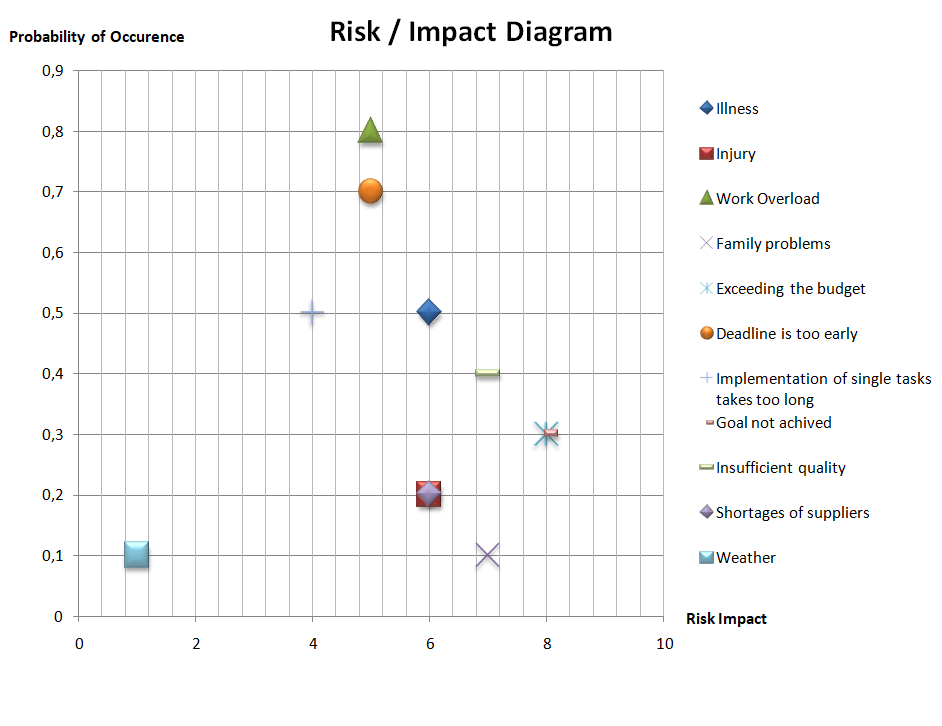
\includegraphics[width =1.1\textwidth]{images/risk-impact2.PNG}
	\caption{Risk/Impact diagram}
	\label{risk-impact}
\end{figure}
The diagram in figure \ref{risk-impact} shows the probability of occurence of the individual risks compared to the possible impact on the project. The impact is evaluated on a scale of 1 to 10. 1 stands for a small but manageable inconvenience, while a 10 represents a threat to the success of the entire project.
\\
As the figure shows, for example, the risk of bad weather poses hardly any threat to the success of the project. A failure to achieve the project's objective however would have far greater impact. Moreover, since the project team consists of only three people, the risks of illness, accidents or other personal problems of the employees were also rated with a large impact. In a project of this size, exceeding the budget would probably have a greater impact on customer satisfaction and thus on the success of the project.

\section{Response to the risk}

\subsection{Project Managment Report [Prmr]}
\label{sec:orgd96ec13}
\begin{center}
\begin{tabular}{|l|r|}
	\hline
	 & Time in hours\\
	 \hline
	optimistic & 65\\
	\hline
	most likely & 92\\
	\hline
	pessimistic & 130\\
	\hline
\end{tabular}
\end{center}
\begin{itemize}
\item create product requirement catalog (50 / 70 / 100)
\item create GANTT diagram (5 /10 / 15)
\item negoitate time and costs with customer (10 / 12 /15 )
\end{itemize}

\subsection{Hardware prerequisites [Hpre]}
\label{sec:orgfb33f5b}

\begin{center}
	\begin{tabular}{|l|r|}
		\hline
		& Time in hours\\
		\hline
		optimistic & 108\\
		\hline
		most likely & 182\\
		\hline
		pessimistic & 256\\
		\hline
	\end{tabular}
\end{center}


\subsubsection{Video cameras [HpreCam]}
\label{sec:org3a27049}
	\begin{enumerate}
	\item research for good product
	\begin{itemize}
	\item investigate environment / areas / building (8/10/12)
	\item estimate amounts and total costs (8/10/12)
	\end{itemize}
	\item negotiate with customer (8/10/12)
	\item buy those products (8/10/12)
	\end{enumerate}

\subsubsection{Storage [HpreS]}
\label{sec:orgeb93f9e}
\begin{enumerate}
\item research archive backup file system
\begin{itemize}
\item NAS with redundance (RAID 2) (4/6/8)
\item Backup also with (RAID 2) (4/6/8)
\end{itemize}
\end{enumerate}

\subsubsection{Panels [HpreP]}
\label{sec:org4b41c6c}
\begin{enumerate}
\item research for good product
\begin{itemize}
\item investigate environment / areas / building (8/10/12)
\item estimate amounts and total costs (4/8/12)
\end{itemize}
\item negotiate with customer (4/8/12)
\item buy those products (4/8/12)
\end{enumerate}

\subsubsection{Control Unit (PLC) [HprePLC]}
\label{sec:orgd40ef86}
\begin{enumerate}
\item research for good product
\begin{itemize}
\item investigate environment / areas / building (4/8/12)
\item estimate amounts and total costs (4/8/12)
\end{itemize}
\item negotiate with customer (4/8/12)
\item buy those products (4/8/12)
\end{enumerate}

\subsubsection{Server [HpreSer]}
\label{sec:org7b31fb6}
\begin{enumerate}
\item research for good product
\begin{itemize}
\item investigate environment / areas / building (4/8/12)
\item estimate amounts and total costs (4/8/12)
\end{itemize}
\item negotiate with customer (4/8/12)
\item buy those products (4/8/12)
\end{enumerate}
\subsubsection{Sensors [HpreSens]}
\label{sec:org6352bec}

\begin{enumerate}
\item research for good product
\begin{itemize}
\item investigate environment / areas / building (4/8/12)
\item estimate amounts and total costs (4/8/12)
\end{itemize}
\item negotiate with customer (4/8/12)
\item buy those products (4/8/12)
\end{enumerate}



\subsection{Hardware installation [Hin]}
\label{sec:org2cae8f9}

\begin{center}
\begin{tabular}{|l|r|}
	\hline
	& Time in hours\\
	\hline
	optimistic & 40\\
	\hline
	most likely & 50\\
	\hline
	pessimistic & 60\\
	\hline
\end{tabular}
\end{center}

\subsubsection{installation and configuration}
\label{sec:org7c12187}
\begin{itemize}
\item video cameras (8/10/12) [HinCam] 
	\begin{itemize}
	\item dependent on [HpreCam]
	\end{itemize}
\item storage  (8/10/12)[HinS]
	\begin{itemize}
	\item dependent on [HpreS, HpreCam]
	\item connect video cameras to system
	\end{itemize}
\item panels (8/10/12)[HinP]
	\begin{itemize}
	\item dependent on [HpreP]
	\item configuration
	\end{itemize}
\item Control Unit (PLC) (8/10/12) [HinPLC]
	\begin{itemize}
	\item dependent on [HpreP]
	\end{itemize}
\item Sensors (8/10/12) [HinSens]
	\begin{itemize}
	\item dependent on [HpreSens]
	\end{itemize}
\end{itemize}

\subsection{Software prerequisites [Spre]}
\label{sec:org180caa5}

\begin{center}
\begin{tabular}{|l|r|}
	\hline
	& Time in hours\\
	\hline
	optimistic & 2\\
	\hline
	most likely & 8\\
	\hline
	pessimistic & 16\\
	\hline
\end{tabular}
\end{center}

\subsubsection{Matlab [SpreMat]}
\label{sec:orgda25cf6}
\begin{itemize}
\item Buy licence / install software  (1/4/8)
\end{itemize}

\subsubsection{PLC IDEs - Automation Studio [SprePLC]}
\label{sec:org003d4a8}
\begin{itemize}
\item Buy licence / install software (1/4/8)
\end{itemize}

\subsection{Software [So]}
\label{sec:orgdf36b5c}

\begin{center}
\begin{tabular}{|l|r|}
	\hline
	& Time in hours\\
	\hline
	optimistic & 604\\
	\hline
	most likely & 810\\
	\hline
	pessimistic & 1259\\
	\hline
\end{tabular}
\end{center}
\subsubsection{create infrastructure [SoInf]}
\label{sec:org06c00a2}
\begin{itemize}
\item setup wiki (1/4/8)
\item setup slack (1/2/3)
\item setup git respository (1/2/3)
\item setup task managment (1/2/3)
\end{itemize}
\subsubsection{System analysis [SoAn]}
\label{sec:org498acda}
\begin{itemize}
\item design architecture (24 / 30 / 48)
\item define components / communication with external systems (interfaces) (24 / 30 / 48)
\item invastigate time in finding out what technologies we want to use (24 / 30 / 48)
\item create diagrams(24 / 30 / 48)
\item describe behaviour of components and depedencies (24 / 30 / 48)
\item find out problematic and time consuming tasks and challanges (24 / 30 / 48)
\end{itemize}
\subsubsection{System design [SoDes]}
\label{sec:org1137d7c}
\begin{itemize}
\item design mutliple GUI and Usability concept (48 / 60 / 90 )
\item gather feedback from customer and redesign concepts (48 / 60 / 90 )
\item design prototyp with fake data (48 / 60 / 90 )
\end{itemize}
\subsubsection{System implementation [SoImpl]}
\label{sec:orgf2f809f}
\begin{itemize}
\item implement components (200 / 300 / 480)
\item unit tests (24 / 30 / 48)
\item integration test (24 / 30 / 48)
\item E2E testing (24 / 30 / 48)
\item documentation (40 / 50 / 60)
\end{itemize}



\subsection{Delivery [Dlvry]}
\label{sec:org1388080}
\begin{center}
\begin{tabular}{|l|r|}
	\hline
	& Time in hours\\
	\hline
	optimistic & 13\\
	\hline
	most likely & 30\\
	\hline
	pessimistic & 50\\
	\hline
\end{tabular}
\end{center}
\begin{itemize}
\item present / demonstrate system and software (12 / 20 / 30)
\item get customer approval (1 /10 / 20)
\end{itemize}

\subsection{Precedence Chart}
\begin{figure}[h]
	\centering
	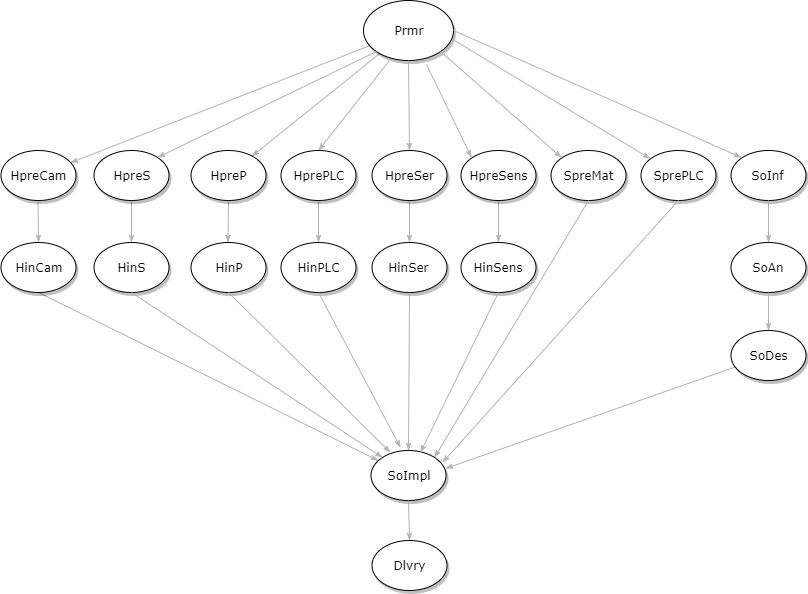
\includegraphics[width=\textwidth]{images/precedenceChart}
\end{figure}


\chapter{Product and Cost Analysis}
\label{market-analysis}
The Care Home is a facility that attaches great importance to safety and energy efficiency. Therefore, it is essential to check different products for certain characteristics. The following attributes are particularly important.
\begin{itemize}
	\item power consumption (sustainability)
	\item costs
	\item integration with systems
	\item compatibility
	\item maintainability
	\item lifespan
	\item customer support 
\end{itemize}

%=================================================================================
\section{Surveillance camera}
By taking the criteria into account, the closer decision was made on two models. The \textit{Bascom Pro Dom-Camera} and the \textit{Sony IP SNC-EB632R}. Dome cameras are semicircular and can be mounted on the ceiling or on a roof (as opposed to bullet cameras). Dome cameras also attract less attention. Bacom's Dome camera uses wireless data transmission and can be connected to the regular power supply. The Sony camera can be powered via Ethernet (power over ethernet) and also provides data via the same cable. Both have an IP66 standard. Thus they can be used inside as well as outside of the building. There is hardly any difference in price, which is why this does not contribute to the purchase decision. However, the wired version is more reliable as signal interference has less influence on the quality. Therefore, the first choice is the Sony camera.
\begin{figure}[h]% 
	\centering 
	\subfloat[Bascom Dome Camera]{ 
		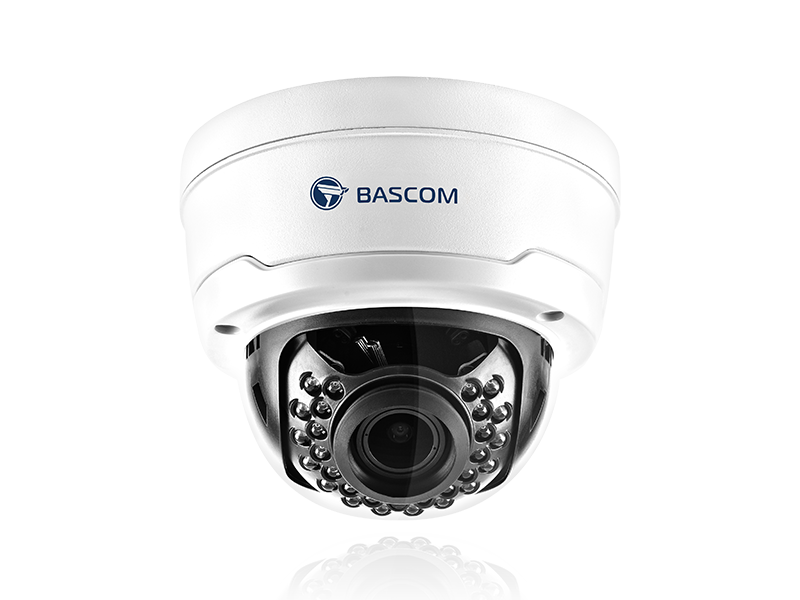
\includegraphics[width=0.4\textwidth]{images/CostAnalysis/domeCamera-pd20}% 
	} \hspace{1cm}
	\subfloat[Recorder for Dome Camera]{ 
		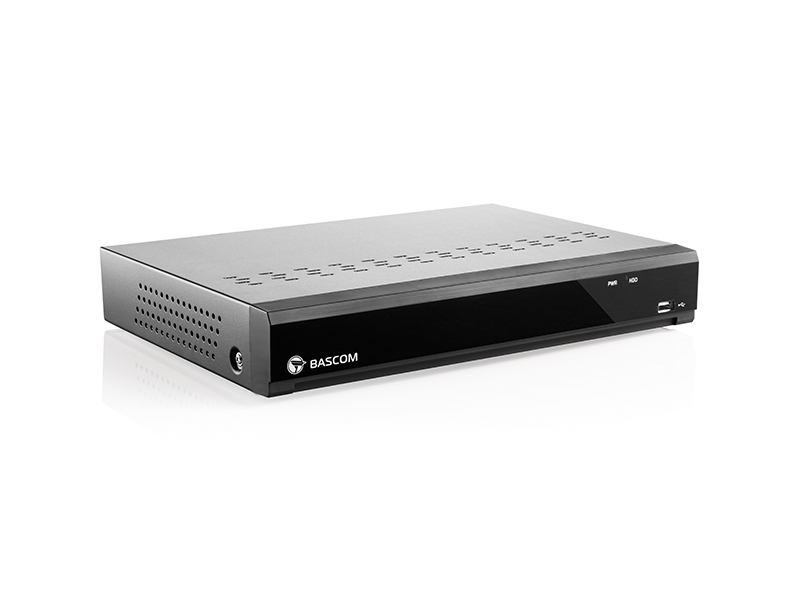
\includegraphics[width=0.4\textwidth]{images/CostAnalysis/recorder-pr4}% 
	} 
	\caption{Dome Camera System}% 
	\label{fig:domeCameraSystem}% 
\end{figure}

\begin{figure}[h]
	\centering
	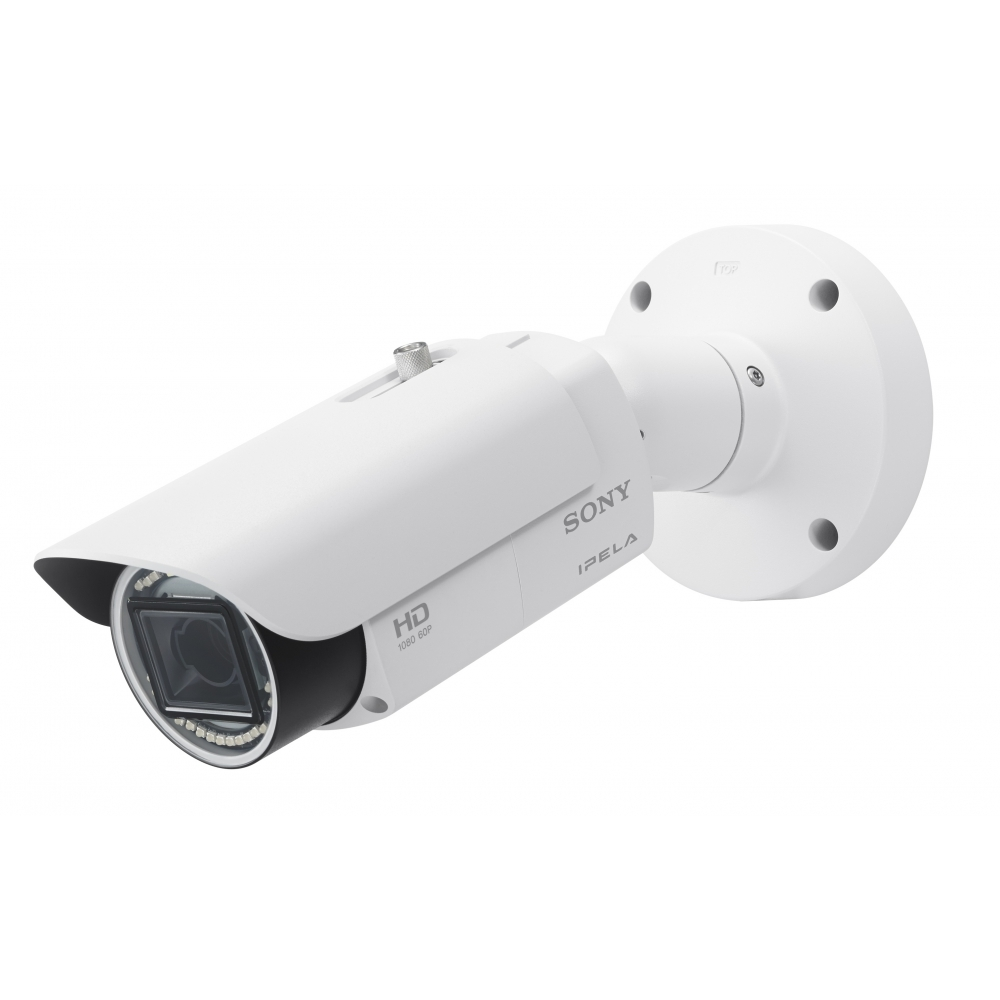
\includegraphics[width=.5\textwidth]{images/CostAnalysis/sony-ip-bullet-kamera} 
	\caption{Sony IP Bullet Camera}
	\label{fig:sonyCamera}
\end{figure}

%=================================================================================
\section{Smoke detector}
In the event of a fire, it is essential to have reliable smoke detectors in operation. Since this project aims to score points above all with customer satisfaction, inconspicuous and simple smoke detectors are preferable. There are several manufacturers that produce, for example, smart smoke detectors. Examples are Bosch, Nest or innogy. Smart devices have the advantage of being relatively easy to integrate into a system. The data can be retrieved via Wifi, Bluetooth or via web app. It is even possible to integrate the functions of the smoke detector into your own application via the API.
\\
Considering the above mentioned criteria, the choice was made for the second generation of the \textit{Nest Protect}. It scores with its simple appearance and the variety of functionality.  The price and performance of this device match very well and outperform the competition.

\begin{figure}[h]
	\centering
	
\includegraphics[width=.4\textwidth]{images/CostAnalysis/NestProtect} 
	\caption{Nest Protect Smoke Detector}
	\label{fig:smokeDetection}
\end{figure}

%=================================================================================
\section{NAS }
The network hard disk is a device that must function reliably. Important data is stored there and must be quickly accessible. That's why sufficient RAM (at least 8 GB) and a modern processor is of great importance. Another important point is of course the scalability, as well as the integration into the system, and commissioning.
\clearpage
\begin{figure}[h]
	\centering
	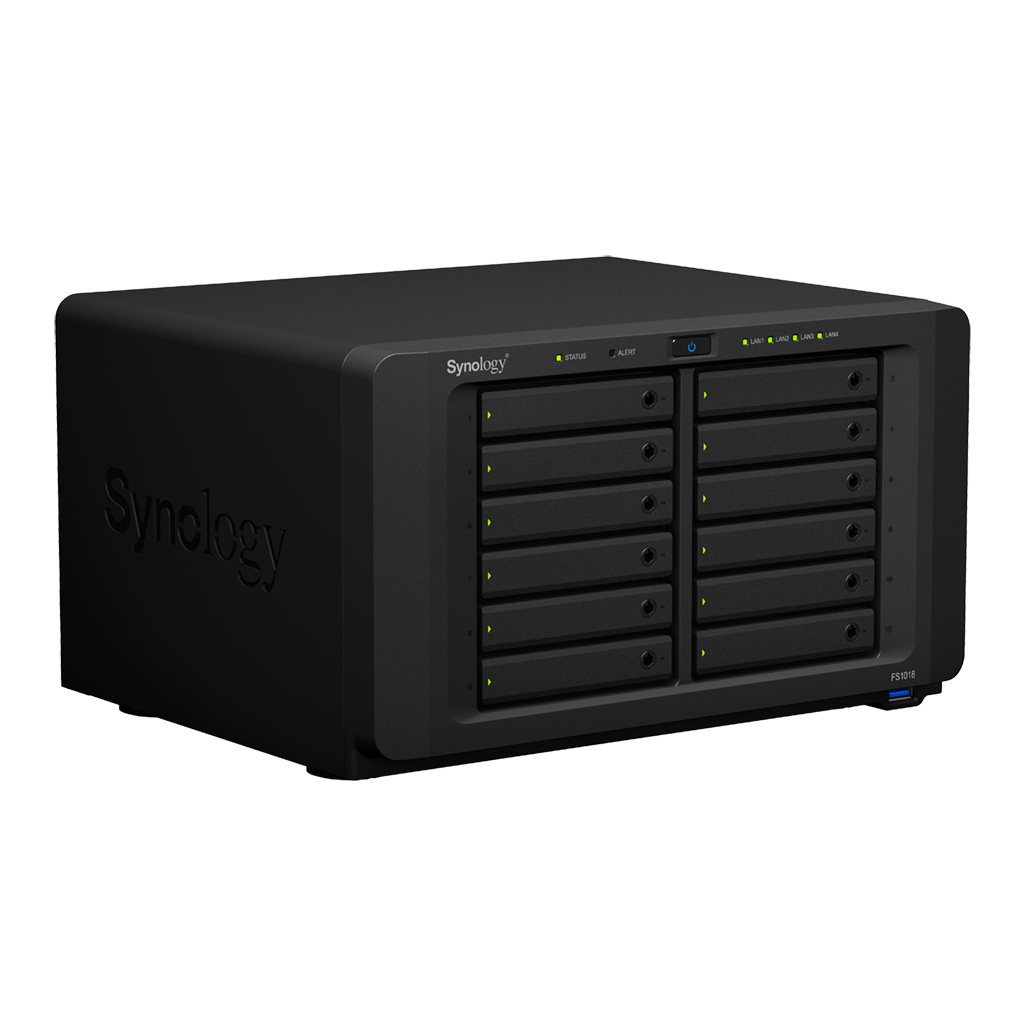
\includegraphics[width=.6\textwidth]{images/CostAnalysis/synologyFS1018} 
	\caption{NAS}
	\label{fig:nas}
\end{figure}

At this point, the \textit{Synology FlashStation FS1018} was chosen. With 12 SSD disks, it has sufficient storage capacity to store the most important data over a long period of time. The specifications are also appealing. Synology advertises their product with low latency, which is important for the application because emergency data, for example, must be retrieved quickly.

%=================================================================================
\section{Inductive and smart sensors}
In this application, inductive sensors are required to obtain the status of different furnishing objects. Examples of this are e. g. whether a door or a window is open or closed. Inductive sensors are available in different sizes, from different manufacturers. However, the choice fell on a certain sensor from Sick. The \textit{Sick IME08-1B5PSZT0S} is an inconspicuous and reliable proximity sensor that fits well into our concept. 
\newpage
\begin{figure}[h]
	\centering
	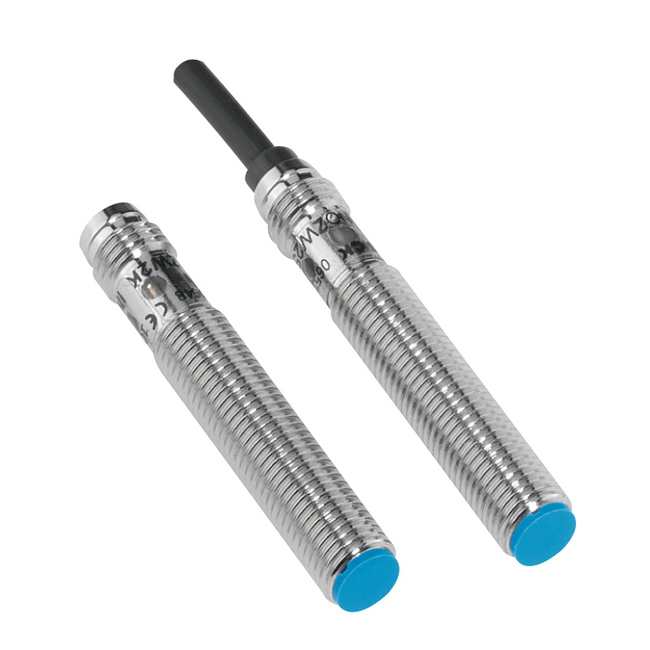
\includegraphics[width=.4\textwidth]{images/CostAnalysis/sickIni} 
	\caption{Sick inductive sensor}
	\label{fig:sickIni}
\end{figure}

Another idea is to use a smart sensor instead of an inductive sensor. The smart heating system (chapter \ref{sec:smartHeating}) enables these two systems to interact with each other in order to create an efficient cooperation. A certain smart door and window contact from Panasonic has stood out. The \textit{Panasonic KX-HNS101}.

\begin{figure}[h]
	\centering
	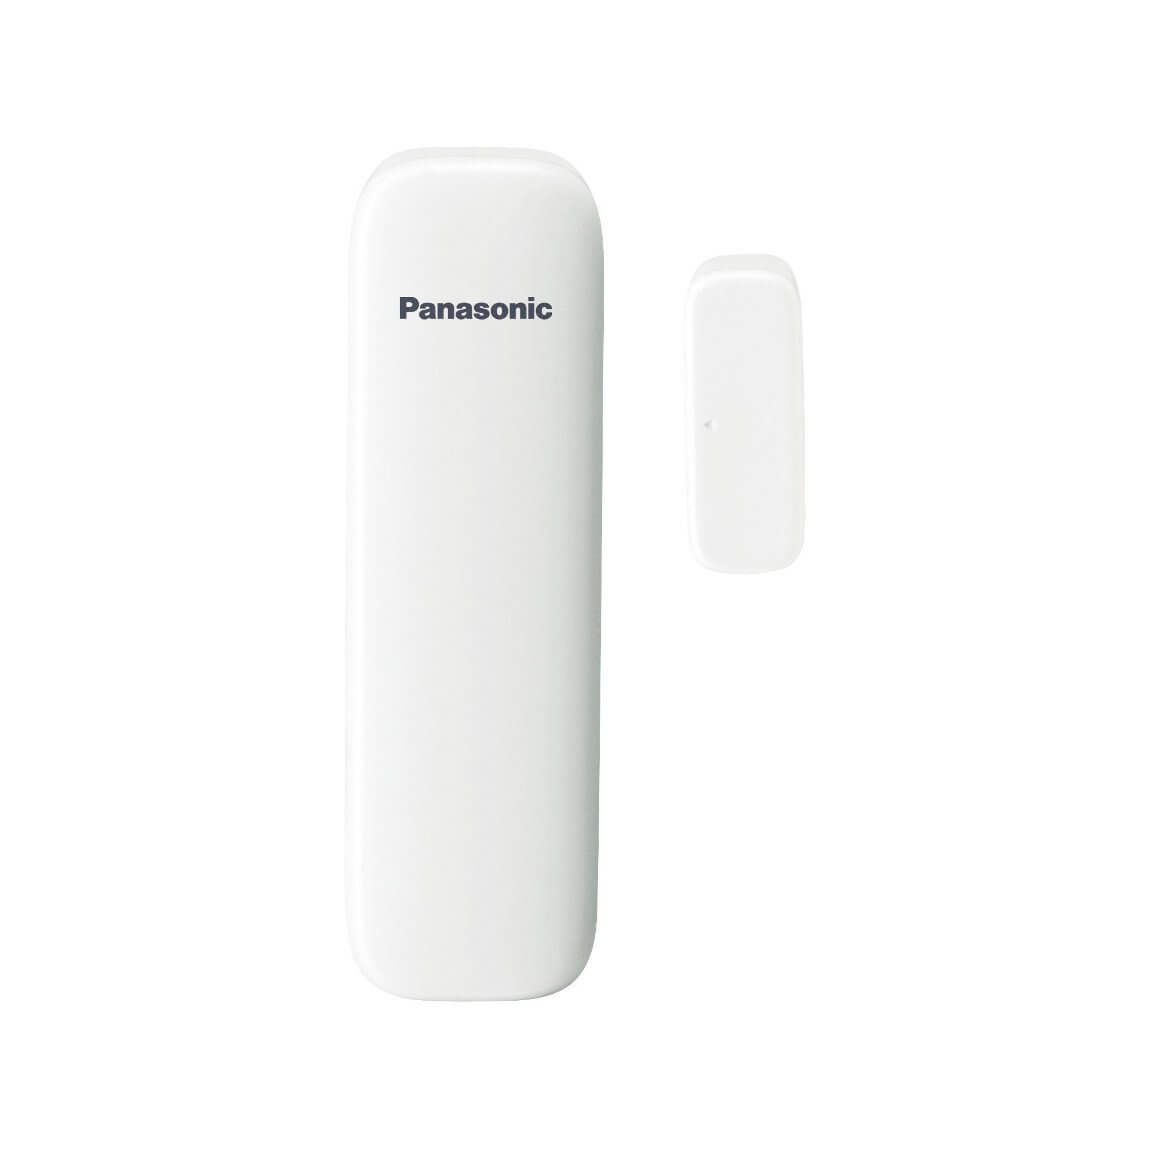
\includegraphics[width=.4\textwidth]{images/CostAnalysis/panasonicfensterkontakt} 
	\caption{Sick inductive sensor}
	\label{fig:panasonicSmart}
\end{figure}

%=================================================================================
\section{Database Server}
An important aspect of this project is the storage of data in a database. For this it is important that it is both scalable and robust. Data must be transported quickly and securely. And a lot of memory must be available. The \textit{Dell EMC PowerEdge T640} was selected for this. Because it is a tower server and not a server for the rack, the consumption is lower, which fits our needs for this project.

\begin{figure}[h]
	\centering
	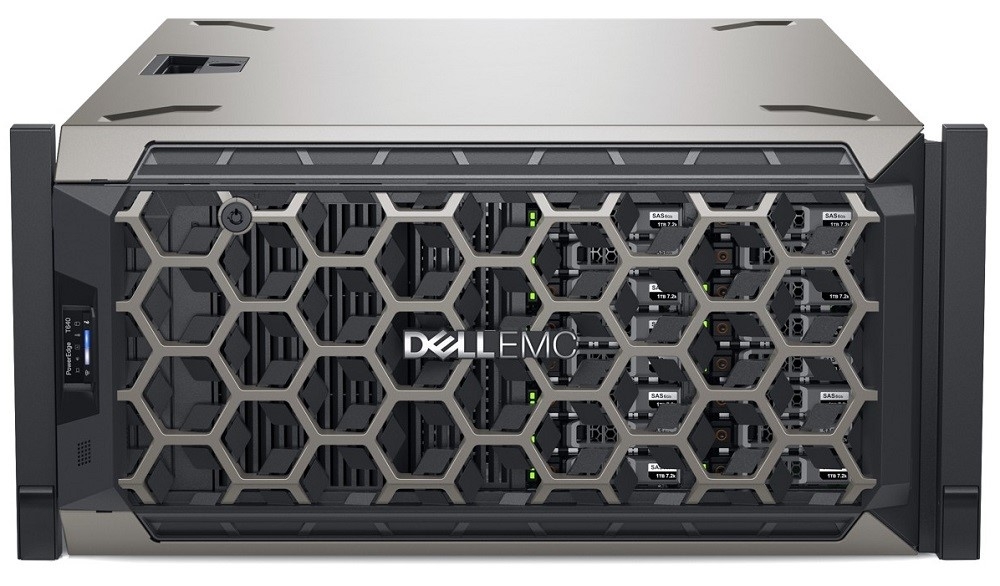
\includegraphics[width=.6\textwidth]{images/CostAnalysis/DellEMCPowerEdgeT640} 
	\caption{Dell EMC PowerEdge T640}
	\label{fig:dbServer}
\end{figure}

%=================================================================================
\section{CPU for PLC System}
PLC systems are used to process sensor data and send signals to devices. In this way, controllers can be written that receive, process sensor data and supply outputs that control actuators. This can be used to realize comfort functions. When a sensor receives a certain value, an actuator is activated which automatically opens doors or switches lights on or off, for example. Since we gained a lot of positive experience with B\&R through other projects, the choice was made for the \textit{X20CP1485 CPU}. It is characterised by its compact size, low energy consumption and extensibility. It is also capable of supporting various protocols such as POWERLINK or CAN. Thus we are flexible in development and can react dynamically to hardware changes.

\begin{figure}[h]
	\centering
	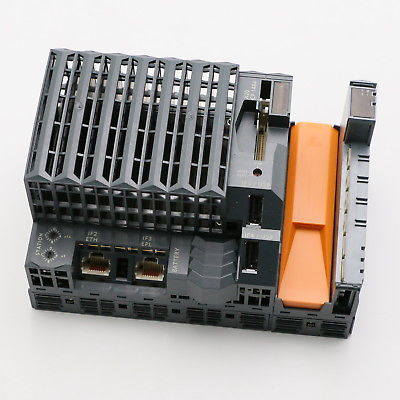
\includegraphics[width=.5\textwidth]{images/CostAnalysis/BR-Automation-X20-CP-1484} 
	\caption{B\&R CPU}
	\label{fig:brCPU}
\end{figure}

%=================================================================================
\section{Motion detectors}
Motion detectors are an important part of our application. Since mostly elderly people live in the care home, it is important that they come into contact with technical equipment as little as possible. This increases the comfort factor enormously. They do not have to deal with technical innovations, but can enjoy their stay. The motion detectors are required to control lights, for example, when a resident is in a certain area. Since we don't want the residents to feel observed, the motion detector must be very simple. It must not interfere with the environment or be technically impaired by the exterior. Since there are also many manufacturers with good equipment like Philips, Elgato or Lupusec, the choice is not easy. The price-performance ratio and simplicity are an important point. That's why we chose the \textit{Lupusec DUAL Way}.
\newpage
\begin{figure}[h]
	\centering
	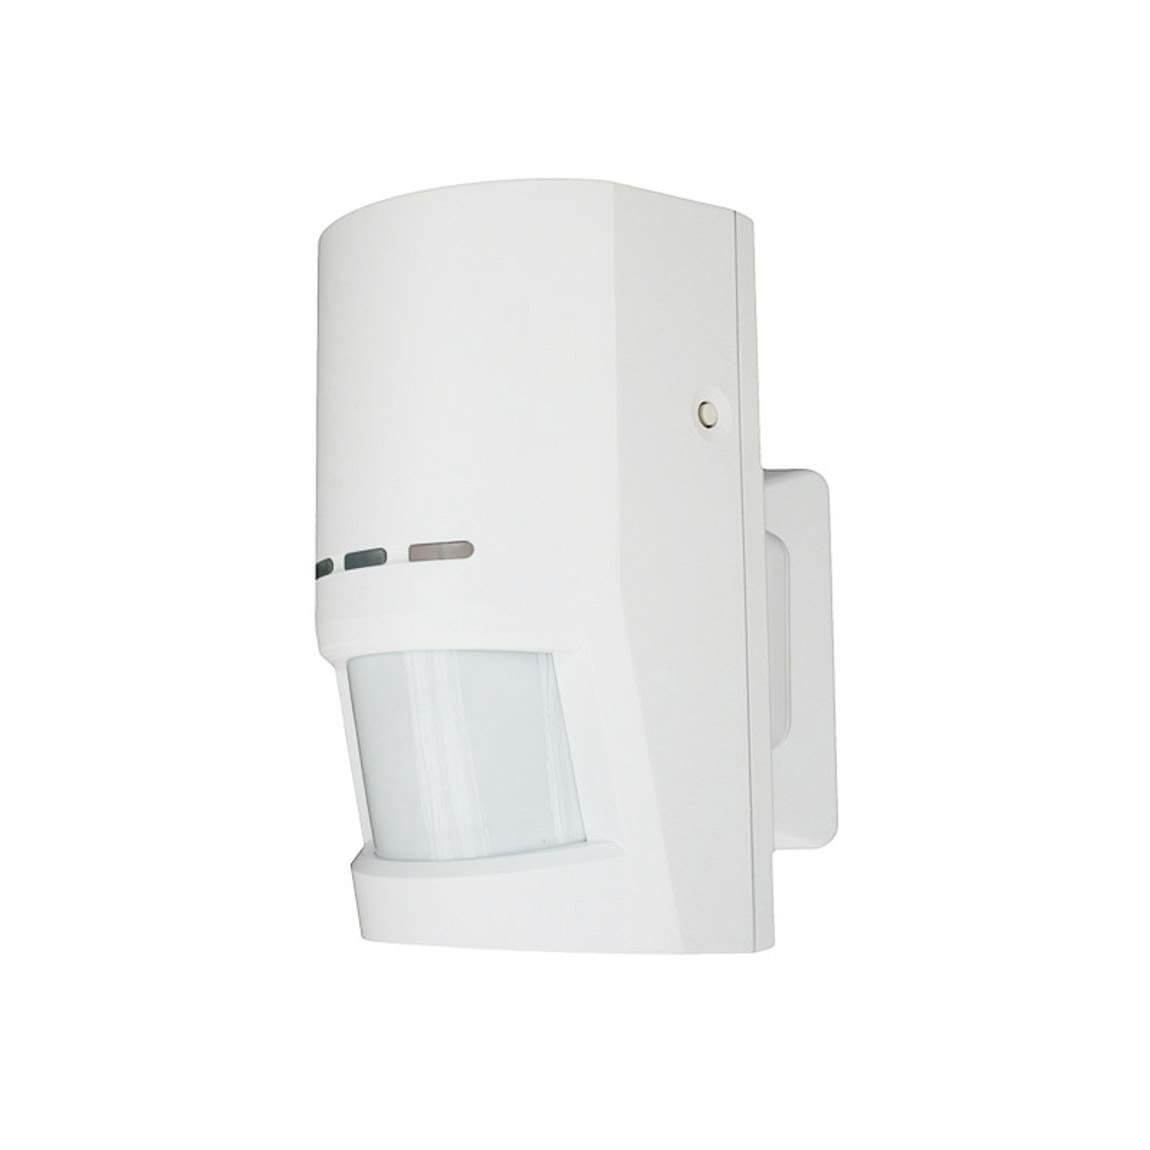
\includegraphics[width=.4\textwidth, trim=3cm 3cm 3cm 4cm, clip]{images/CostAnalysis/lupusecBewegungsmelder} 
	\caption{Lupusec DUAL Way}
	\label{fig:lupusecDual}
\end{figure}

%=================================================================================
\section{Healthcare Wristband}
A constant control of body values for patients can be very helpful to the caregivers. Classical methods such as pulse measurement or blood pressure measurement must be done manually by helpers and cost the patient time. During this time they are often not allowed to move, otherwise they can influence the values. Long-term measurements with old devices are complex and error-prone and do not give the patient a good and relaxing feeling. Our aim is to carry out long-term measurements, which the patient does not notice in the best case scenario. We use the \textit{Lenovo HW01 Smart Wristband}, which comes with a variety of features. 
\begin{itemize}
	\item pedometer
	\item sleep monitor
	\item heart rate measurement
	\item Date and time
	\item wake-up function
	\item stopwatch
	\item notifications
	\item Music playback control
	\item movement memory
	\item GPS run mode
\end{itemize}
Of course, this device does not replace special medical devices. However, it can be used for forecasting and unobtrusive monitoring, which can react quickly in an emergency.

\begin{figure}[h]
	\centering
	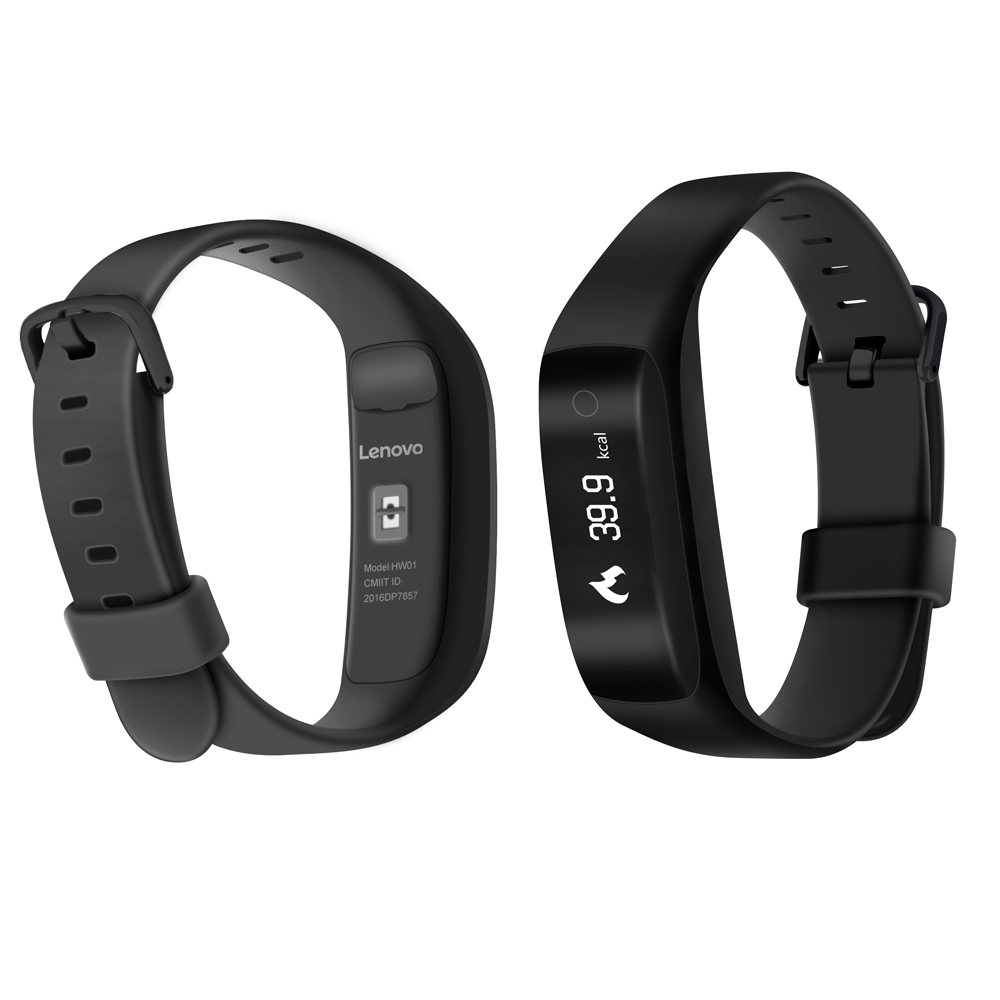
\includegraphics[width=.5\textwidth, trim=1cm 4cm 2cm 4cm, clip]{images/CostAnalysis/LenovoHW01} 
	\caption{Lenovo HW01 Smart Wristband}
	\label{fig:lenovoHealth}
\end{figure}

%=================================================================================
\section{Emergency button}
In order to offer patients the possibility to submit a message in case of emergency, we have decided to implement an emergency button. The data is then stored and evaluated centrally to prevent emergencies from being simulated or inadvertently activated. The \textit{FIBARO The Button (Z-Wave)} is a good and efficient way to realize this idea.
\newpage
\begin{figure}[h]
	\centering
	
\includegraphics[width=.4\textwidth]{images/CostAnalysis/fibaroEmergency} 
	\caption{FIBARO The Button (Z-Wave)}
	\label{fig:fibaroEmergency}
\end{figure}

%=================================================================================
\section{Smart heating system}
\label{sec:smartHeating}
A very important point in our product development is the heating of rooms. A lot of energy is lost there if the heating is not efficient. One of the market leaders in smart heating is the manufacturer Elgato. The product of our choice is the \textit{second-generation Elgato Eve Thermo}. 
\\
In addition to a simple installation, simple appearance and display, it comes with a variety of useful functions. Schedules can be set for heating schedules. It is also possible to view a consumption analysis. Both for the heating behaviour and for the energy. Another useful feature is the possibility to connect doors and window sensors with the smart heating system. As a result, the system knows when the windows and doors are opened and can regulate the heating process efficiently.
\newpage
\begin{figure}[h]
	\centering
	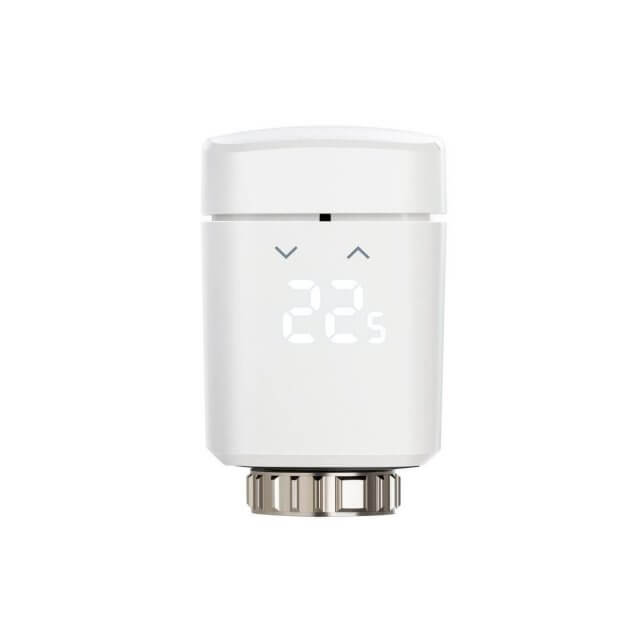
\includegraphics[width=.5\textwidth, trim=0 3cm 0 3cm, clip]{images/CostAnalysis/elgato-eve-thermo} 
	\caption{Elgato Eve Thermo}
	\label{fig:elgatoEve}
\end{figure}

%=================================================================================
\section{Water consumption}
A very important point in the care home system is the analysis and monitoring of water consumption. The data should be collected automatically and forwarded to a central point so that water consumption can be regulated. Abnormal behaviour can also be detected, for example, if someone has forgotten to turn off the water. In this case, warning signals can be sent to the staff to check that everything is in order and can act quickly in an emergency. A very interesting product is the \textit{FLUID meter}, which is used in our project.

\begin{figure}[h]
	\centering
	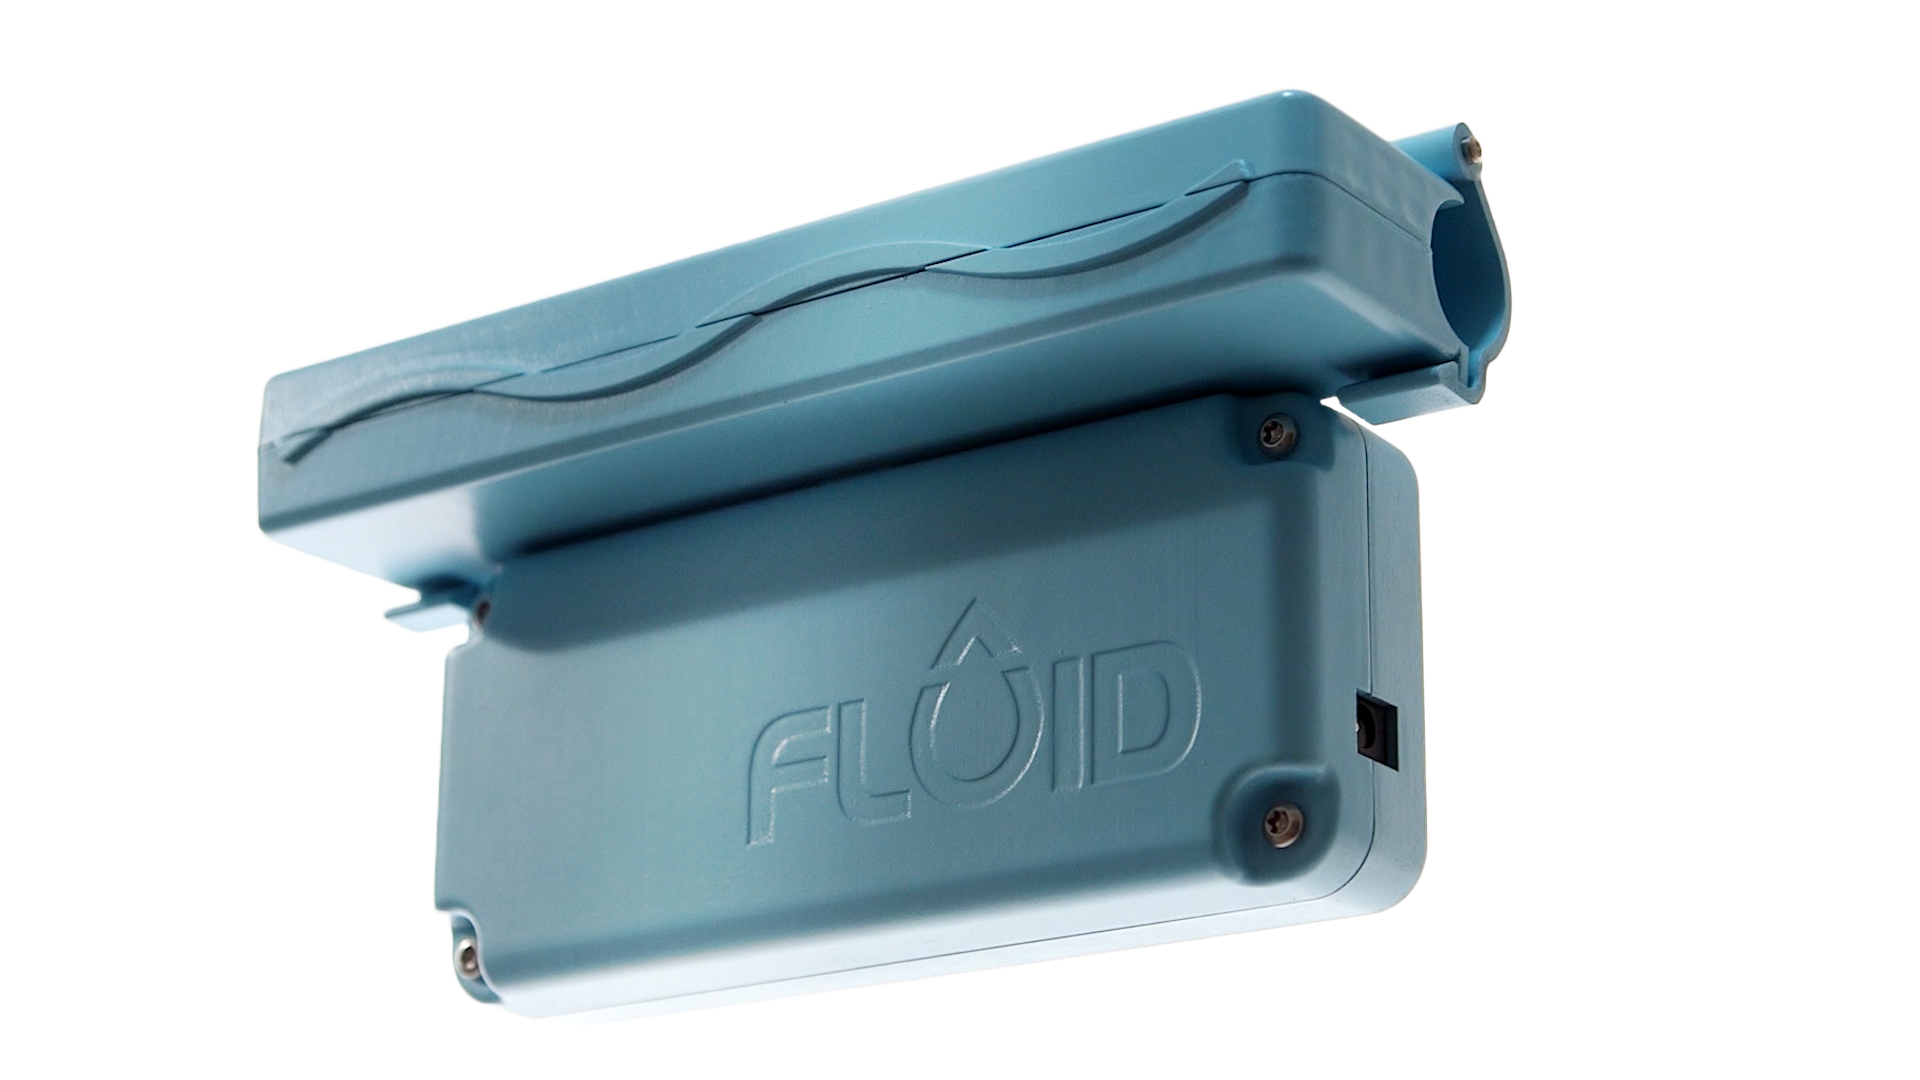
\includegraphics[width=.6\textwidth]{images/CostAnalysis/fluidMeter} 
	\caption[FLUID meter]{FLUID meter\protect\footnotemark}
	\label{fig:fluidMeter}
\end{figure}
\footnotetext{Source:\\http://www.fluidwatermeter.com/wp-content/uploads/2014/11/Fluid-Campaign.00\_00\_57\_18.Still002.png}
%=================================================================================
\section{HMI Tablets}
It makes sense to use a portable tablets to transfer information quickly to the staff. The idea is that nurses can digitally enter and retrieve patient records. With one click statistics about patients and rooms can be retrieved and managed. Another use case is that the cleaning staff has a possibility to document the cleaned rooms. Things like cleanliness or contamination can be noted. Our product of choice is the \textit{iPad Pro}, which scores points for its performance and simple appearance. Although it is more expensive than the competition, we have had good experiences with these tablets in the past, which has made our decision easier.
\\
\\
\begin{figure}[h]
	\centering
	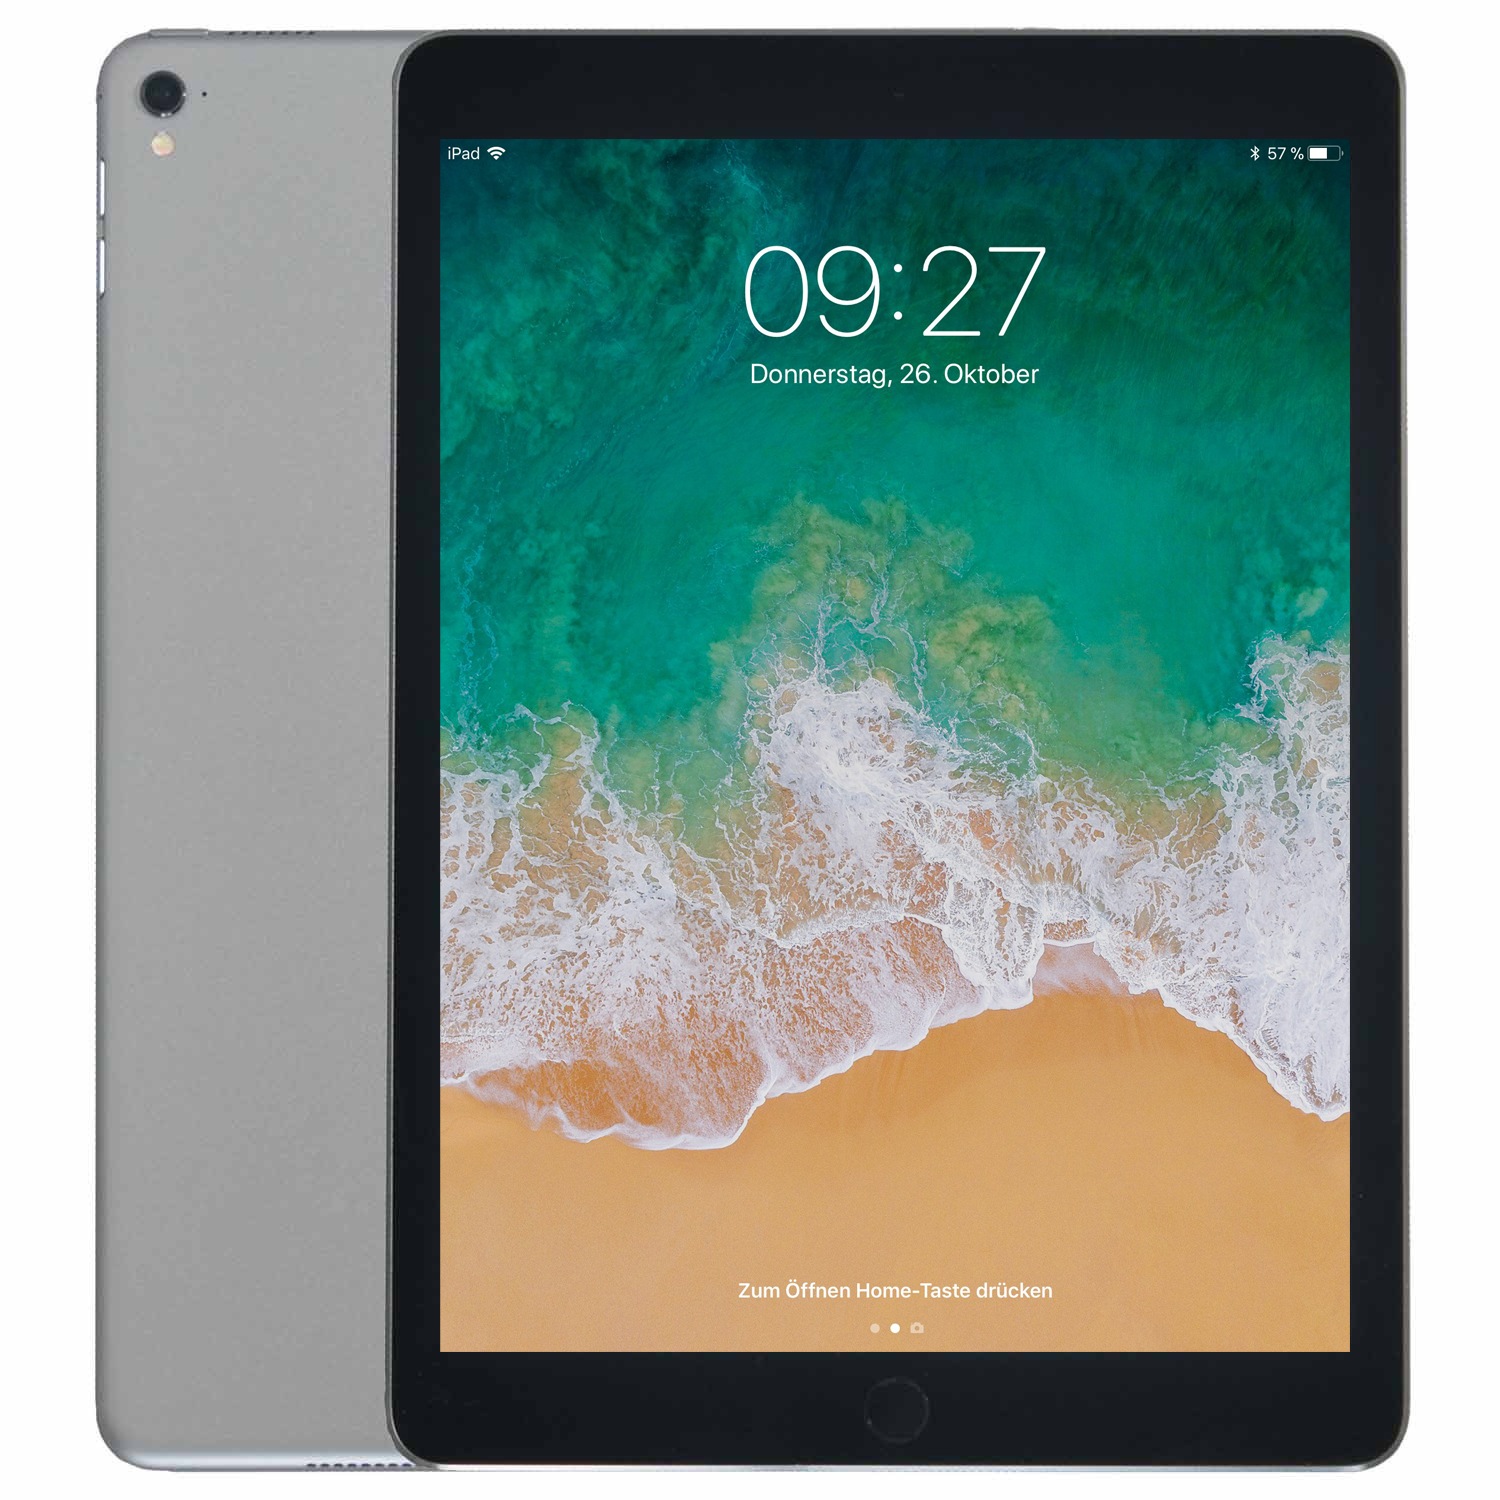
\includegraphics[width=.5\textwidth]{images/CostAnalysis/iPadPro} 
	\caption[12,9" iPad Pro]{12,9" iPad Pro\footnotemark}
	\label{fig:iPadPro}
\end{figure}
\footnotetext{Source: \\https://media.nbb-cdn.de/images/products/310000/316143/Apple\_iPadPro\_2017\_space\_Hero.jpg}
\clearpage
%=================================================================================
\section{Cost Calculation}
\begin{table}[h]
	\centering
	\renewcommand{\arraystretch}{1.9}
	\begin{tabular}{lrrr}
	Label & Price Per Unit [\officialeuro] & Amount & Cumulative Costs [\officialeuro] \\
	\hline
	Sony IP SNC-EB632R & 1,000 & 5 & 5,000\\
	Nest Protect & 130 & 120 & 15,600\\
	Synology FlashStation FS1018 & 1,600 & 2 & 3,200\\
	Panasonic KX-HNS101 & 30 & 250 & 7,500\\
	Dell EMC PowerEdge T640 & 2,000 & 2 & 4,000\\
	B\&R X20CP1485 & 2,000 & 2 & 4,000\\
	Lupusec DUAL Way & 200 & 160 & 32,000\\
	Lenovo HW01 Smart Wristband & 30 & 120 & 3,600\\
	FIBARO The Button (Z-Wave) & 50 & 110 & 5,500\\
	Elgato Eve Thermo 2. Gen & 80 & 110 & 8,800\\
	FLUID meter & 250 & 130 & 32,500\\
	12,9" iPad Pro & 1,000 & 20 & 20,000\\
	\hline
	%Products Total & & & \textbf{xxx}\\
	Working Hours (most likely)& 1172 & 100 & 117,200 \\
	Overhead Costs &  &  & 40,000\\
	\hline
	\hline
	Nett Total & & & 293,905\\
	+ VAT 20\% & & & 58,781\\
	\hline
	\hline
	\textbf{Total} & & & \textbf{352,686}
	\end{tabular}
\end{table}


\chapter{Product development}
This chapter describes the technical side of this project. The technologies used, the network peripherals and the architecture of the iCare system are discussed here.

\section{Basic architecture}
In order to give the user as much freedom as possible and to save him the installation and administration of unnecessary software and unnecessary software components, this project is implemented as a web server. This means that the system can be accessed by every employee under their user ID and password via the Internet using a web browser. The user interface elements are designed to be comfortably operated from a desktop PC as well as from mobile devices such as tablets and smartphones. This makes the iCare system platform independent and supports an easy and elegant user experience. The intention is to make it as easy as possible for the user to use the iCare system by using technologies that every user can use intuitively.

\subsection{iCare Network}
The server uses both wireless connections and the Ethernet connection within the care home to communicate with all connected devices as well as the backup system. As already described in chapter \ref{basic-concept}, each room within the care home has a network HUB, which is connected to the central server via Ethernet. This network HUB communicates either via an Ethernet connection or via a wireless connection with the devices installed in the room. Figure \ref{icare-network} shows the network peripherals of the iCare system:
\begin{figure}[H]
	\centering
	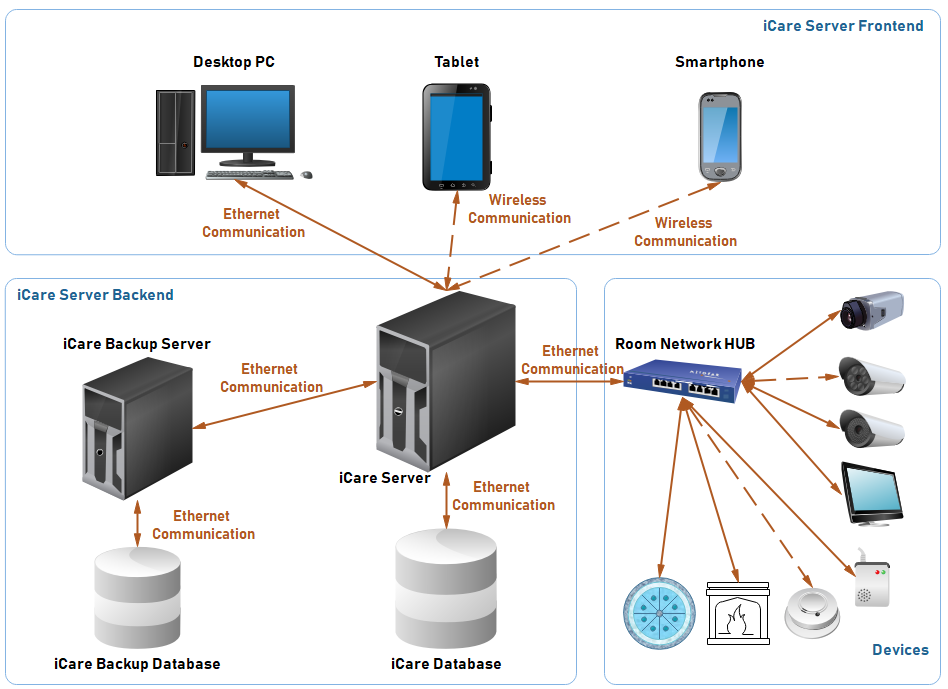
\includegraphics[width =1.0\textwidth]{images/iCare-Network.PNG}
	\caption{iCare Network}
	\label{icare-network}
\end{figure}
The solid lines represent communication via Ethernet cabling, while the dashed lines indicate a wireless connection. The devices connected to the network HUB are already listed in the overview in chapter \ref{basic-concept} for each room and are not considered here. A detailed examination of the individual devices can be found in the hardware calculation in Chapter \ref{market-analysis}.

\subsection{iCare Communication}
The data collected by the devices in the individual rooms is forwarded to the central server via the network HUB. The server analyzes this data, persists it in the database, forwards it to the backup system, and prepares it for display in the frontend of the iCare system. The processed data will also be forwarded to the infoboard for presentation via the network hub of the community room. It is also possible to access and control the devices for central heating and water consumption via the network HUB. For the frontend, it is also possible to send user inputs and user requests to the central server at any time, which then processes them and returns the corresponding results to the frontend. These data and control flows are shown in figure \ref{icare-dataflow}.
\begin{figure}[H]
	\centering
	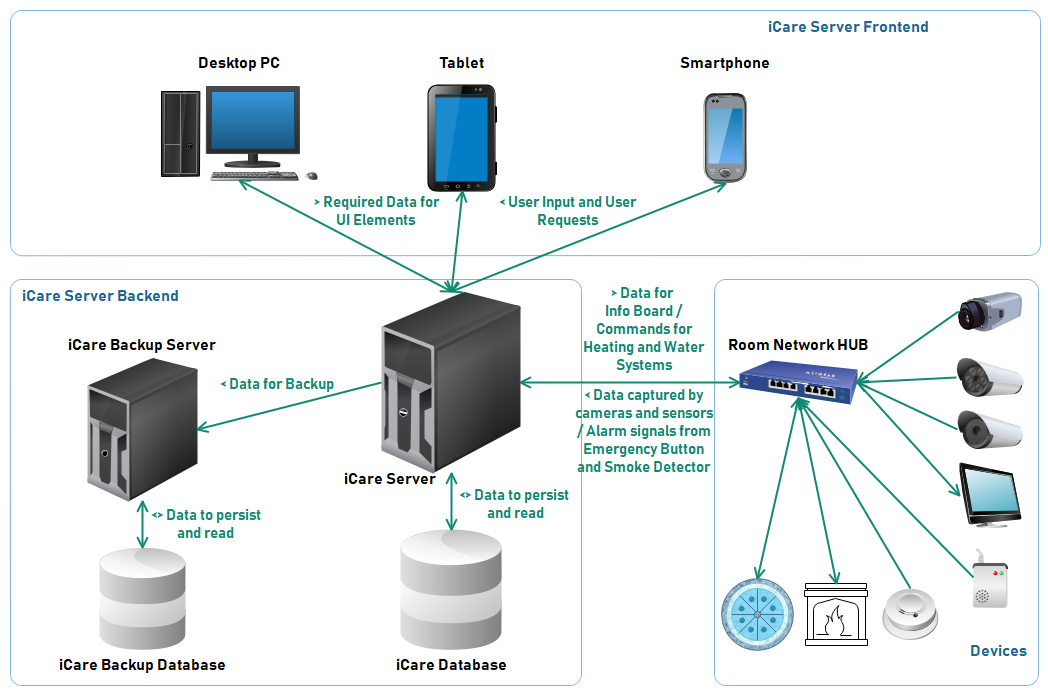
\includegraphics[width =1.05\textwidth]{images/iCare-Dataflow.PNG}
	\caption{iCare control- and data- flows}
	\label{icare-dataflow}
\end{figure}

A more detailed description of the individual subsystems will be given in the next chapters. It focuses on how the communication between the frontend and the backend of the iCare server is implemented, which data model is used, and which features the server offers the user.

\section{Server Backend}
This chapter covers the core component of the iCare Server: The Server Backend. The following subchapters describe the architecture of the server with its individual components and the technologies used to implement communication between the subsystems.
\subsection{The Server architecture}
The following figure \ref{icare-serverarchitecure} shows the general architecture of the backend server and the external systems with which the server communicates at runtime. The focus here lies on the \textit{iCare Server} subsystem, while the other components of the system \textit{iCare Frontend}, \textit{iCare Room HUB}, \textit{iCare Backup System} and \textit{iCare Data} are treated as black boxes. 
\begin{figure}[H]
	\centering
	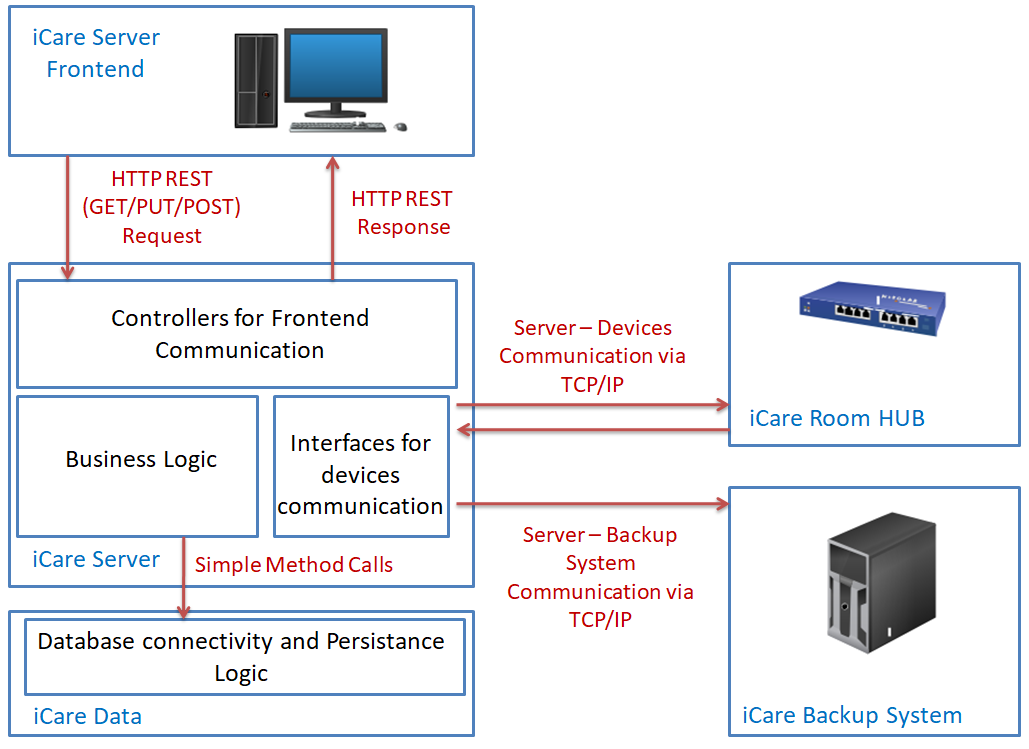
\includegraphics[width =1.0\textwidth]{images/server-architecture.PNG}
	\caption{iCare Server architecture}
	\label{icare-serverarchitecure}
\end{figure}
As can be seen in the picture, the iCare web server has communication interfaces to the other subsystems, which are based on different technologies. The communication between the frontend and the backend is based on Representational State Transfer (REST) web services. The communication with the different devices, which are accessible via a network hub in the individual rooms, works with simple Java sockets. Because the iCare Data module runs on the same system, there is a direct dependency relationship between the iCare Data module and the iCare Server module, enabling the web server to directly access the interfaces of the iCare Data module.
\subsection{Communication between frontend and backend via REST}
As already mentioned, the communication between frontend and backend works via RESTful web services. The web server provides controller classes as access points for the requests of the iCare frontend, which can be reached at the host address of the web server under corresponding extensions. The following address is an example for this kind of access point.
\begin{center}
	\textit{http://www.iCareWeb.de:8080/inhabitant}
\end{center}
The \textit{/inhabitant} access point for example provides a list of all care home residents that carry a wrist band and the corresponding data captured by the wrist band in real time. For example, if the frontend is to display this data in a user interface, a GET request must only be sent to this endpoint at regular intervals. As a response, the frontend receives the current data of all wrist bands packed in a JSON string. The following listing shows one entry in this JSON-String:
\begin{lstlisting}
{
	"id": "a64f3d5c-bade-49f8-b67f-2d5b7d0c55a5",
	"heartRate": 55,
	"name": "Ms. Smith",
	"restrictions": [],
	"healthCheck": {
		"message": "Low heart rate",
		"status": "YELLOW"
	},
	"position": {
		"x": 29,
		"y": 33
	}
}
\end{lstlisting}
How this JSON string is interpreted and displayed lies with the frontend and is not discussed here any further.
\\
The functions for controlling the central heating system can also be called via PUT and POST requests. To do this, a similar JSON string must be packed into the request, which contains the required data. The server then interprets this JSON string and executes the command for the corresponding radiator in the specified room.

\subsection{Communication between Server and Devices/Backup system}
\subsection{Business Logic}
\subsection{Connection to ICare Data}
\chapter{Implementing iCareData}
\label{chap:iCareData}
From the System Designer's point of view, the project is divided into two parts. The building and its inhabitants. 
\\
The iCareData part is called periodically by the server. The tasks are to manage the data of the residents and to define the building. Figure \ref{fig:iCareDataBuilding} on the following page shows the basic structure of the building part. It consists of two interfaces and classes that represent each room in the building. 
\section{Object models}
Each room is a composition of a door as well as bounds. The bounds are important for the building because it contains the architectural measurement of each room. This will also get more important when the building and its inhabitants are displayed on the web page. The door is basically important for the frontend. The position of the doors will make sure, that the inhabitants will walk through them and not through the walls. The two interfaces consist of the coordinates of the entire building and will make sure that every class will implement the right methods.
\begin{figure}[h]
	\centering
	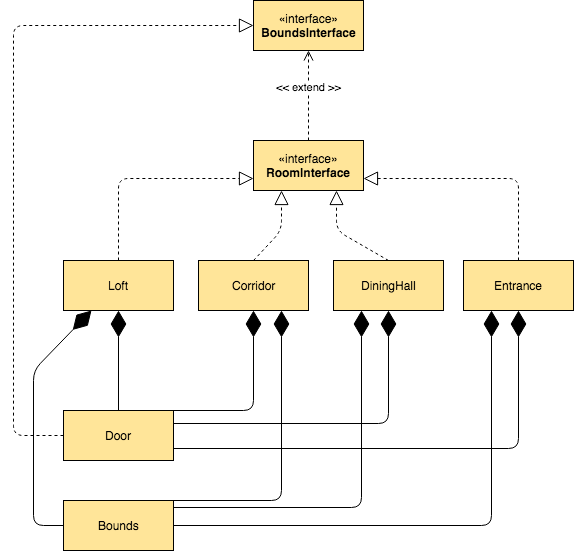
\includegraphics[width=\textwidth]{images/iCareDataBuilding}
	\caption{Object Diagram iCareData Building}
	\label{fig:iCareDataBuilding}
\end{figure}
\clearpage
Figure \ref{fig:iCareDataInhabitant} shows the second part of the iCareData project. It is dedicated to the inhabitants. Each resident is a composition of a healthCheck and a position.
\\
The aim of HealthCheck is to receive the sensor data and make it available to the server as processed data. The data is polled and handled by the CPU from chapter \ref{market-analysis}. For example, if the heart rate comes in a critical state, an alarm is triggered immediately. The data used for this purpose is stored in the resident's object so that it can be displayed on the website. In this way, employees are also visually informed that something is wrong.
\begin{figure}[h]
	\centering
	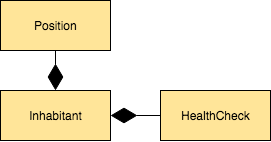
\includegraphics[width=.5\textwidth]{images/iCareDataInhabitant}
	\caption{Object Diagram iCareData Inhabitant}
	\label{fig:iCareDataInhabitant}
\end{figure}
The position is determined as a combination of motion detectors and smart wristbands. However, this is only the case when people need special treatment because they need to be under observation. It is therefore important to know where they are. The information in the healthCheck and the position can be used to determine exactly where a patient is in an emergency.

\section{Mocks}

\section{Implementation - Frontend}

The frontend was implemented with HTML, CSS and Javascript (ES6).
The following open source libraries were used:
\begin{itemize}

\item Chart.js to -  draw the diagrams in the Eco Monitor.
\item Date.js - to manipulate and format dates.
\item P5.js - to draw the interactive tracking interface.
\item Bootstrap 3 - a CSS framework to ensure a modern responsive user interface.
\end{itemize}


The focus in the design was placed on displaying the important messages (alarms) on each page so that staff can always see which new alarms have just been reported.
The user must manually mark these messages as read so that these messages are no longer displayed in the upper right-hand corner. For testing purposes during development, a Develop Tools page was implemented to manually force certain events to test the frontend end-to-end.

\subsection{Dynamic website}
Through timers the frontend calls the backend in the background at regular intervals (1 second), this ensures that the data in the frontend is always up-to-date.

\subsection{Tracking page}
On this page you can see a floor plan of the building showing the positions of the tracked inhabitants.
Every second the points are updated and the corresponding data is updated.
By clicking on a point, the current values of this inhabitant are displayed below the building floor plan ( Heart rate, Health Check, Restrictions, Name and ID).
The colors of the point have been implemented in a traffic light scheme. The dots on the floor plan, each representing an inhabitant, are displayed in these colors accordingly.


\subsection{Dashboard / Notifications}

This page lists the latest notifications in the system in chronological order. 
At the top of the screen, the user also sees additional counters for the various categories: Messages, alerts, tickets and todos. If the user clicks on one of these four fields, a corresponding page appears, which displays the data in more detail.
It was important that an appropriate colour scheme was consistently followed.
Red means urgent information. Yellow, a warning that is not quite as urgent and green means information.
Each notification contains a time stamp, a message, a room in which the event occurred, and the inhabitant, if any.

\subsection{Notification popup}

When a specific event occurs, notifications are sent to the frontend. If the frontend receives a new message, it is stored in an inbox in the frontend. The number of unread notifications is displayed as a red box in the upper right corner of each page of iCare. As soon as at least one unread notification is in the inbox, this red box is displayed. This ensures that important messages do not appear only once and are then missed by the user.
Clicking on this popup takes the user to an overview page in which all unread notifications are listed. With one button, he can set all these messages to read. After that the inbox is empty and the red box is no longer displayed until a new notification arrives.
If notifications are removed from the inbox, they are not deleted, but are still displayed in the recent list in the dashboard.


\subsection{Eco Monitor}

This page provides an overview of the electricity and water consumption of the last 30 days.
In this case, the data is only loaded once when the web page is loaded, since this data does not change as frequently.



\subsection{Camera page}

This page shows the user the last images of the surveillance cameras installed in the Carehome.
At the top he sees the pictures from the reception hall and below the pictures from the outside area. Additionally, a timestamp is diplayed to indicate when the image was taken.

\subsection{Report page}

This page allows you to generate a report for a specified period of time and download it as a pdf file.
The report includes water and electricity consumption. As well as a record of each resident's health check sensors.


\subsection{Settings page}
This page allows you to configure certain settings on the frontend.

\chapter{Customer Feedback}
\label{sec:org4718a3c}

High customer satisfaction is very important to our team. Professor Mousavi also
made it very clear in his lectures that in a good project management the
feedback of the customer is very important. For this reason, the project manager
should regularly request feedback from the customer. We have therefore sent a
survey to our customer three times.

\subsection{Understanding the customer}
\label{sec:org62e7666}
The first survey was mainly about clarifying general questions, so that these can be taken into account in the project
management. Financial topics were addressed specifically and an attempt was made
to bring the features resulting from the specifications into a prioritized
order. This has helped us a lot to focus on
the features that are most important to our customers. The results of the
questions regarding design and performance also gave us conclusions as to which
technologies we should use and how much time we should invest in UI design.
\subsection{Concrete questions relevant for project management}
\label{sec:orgd256524}
\subsubsection{How important for you is to stay below the financial frame given?}
\label{sec:orga929d3d}
Type: Exclusive choice 

CORE: no

Mandatory: yes 

\begin{itemize}
	\item Very important (10)
	\item Important (with possible negotiation if needed) (7)
	\item Important (if it can be reasonably argued) (6)
	\item Not so important (2)
	
	\begin{itemize}
		\item Answer
		\begin{itemize}
			\item Important (with possible negotiation if needed) (7)
		\end{itemize}
	\end{itemize}
\end{itemize}

\subsubsection{Which features are most important to you for the first release? Please prioritize the given features in descending order.}
\label{sec:org7a4b4f5}

Type: Prioritizing 

CORE: no

Mandatory: yes 

\begin{itemize}
	\item Notifications / Alarms
	\item Survailance Cameras
	\item Ticket system
	\item Position Tracking
	\item Health Monitoring
	\item Report generation
	\item Settings to customize UI
	\item Eco Monitoring
	
	\begin{itemize}
		\item Answer
		\begin{itemize}
			\item Notifications / Alarms
			\item Position Tracking
			\item Health Monitoring
			\item Eco Monitoring
			\item Survailance Cameras
			\item Ticket system
			\item Report generation
			\item Settings to customize UI
		\end{itemize}
	\end{itemize}
\end{itemize}

\subsubsection{How important is it to you that the deadline is met?}
\label{sec:orgfcc43e2}
Type: Exclusive choice 

CORE: no

Mandatory: yes 

\begin{itemize}
	\item Very Important (10)
	\item Important (7)
	\item Not so important than creating a good product (5)
	\item Not important (2)
	
	\begin{itemize}
		\item Answer
		\begin{itemize}
			\item Not so important than creating a good product (5)
		\end{itemize}
	\end{itemize}
\end{itemize}

\subsubsection{How important is good usability to you?}
\label{sec:org78edac0}
Type: Exclusive choice 

CORE: no

Mandatory: yes 

\begin{itemize}
	\item Very Important (10)
	\item Important (7)
	\item Less important (5)
	\item Not important (2)
	
	\begin{itemize}
		\item Answer
		\begin{itemize}
			\item Very Important (10)
		\end{itemize}
	\end{itemize}
\end{itemize}

\subsubsection{How important is an aesthetically designed product to you.}
\label{sec:org1dadec1}
Type: Exclusive choice 

CORE: no

Mandatory: yes 

\begin{itemize}
	\item Very Important (10)
	\item Important (7)
	\item Less important (5)
	\item Not important (2)
	
	\begin{itemize}
		\item Answer
		\begin{itemize}
			\item Important (7)
		\end{itemize}
	\end{itemize}
\end{itemize}
\subsubsection{How important is performance to you?}
\label{sec:orgf91a813}

Type: Exclusive choice 

CORE: no

Mandatory: yes 

\begin{itemize}
	\item Very Important (10)
	\item Important (7)
	\item Less important (5)
	\item Not important (2)
	
	\begin{itemize}
		\item Answer
		\begin{itemize}
			\item Important (7)
		\end{itemize}
	\end{itemize}
\end{itemize}


\subsection{Gathering Feedback for the UI Mockups}
\label{sec:orgab0c9bc}
The Email we send to our customers.
\begin{verse}
	\vspace*{1em}
   Dear Ladies and Gentlemen,\\
	\vspace*{1em}
	\vspace*{1em}
	I will send you a selection of logo designs for the iCare software.\\
	Once you have made a selection, we will continue to work out this logo as quickly as possible and send you the new version.\\
	\vspace*{1em}
	We also send you the UI mockups and a survey about them.\\
	\vspace*{1em}
	We look forward to receiving prompt feedback so that we can respond to your wishes as quickly as possible.\\
	\vspace*{1em}
	With kind regards,\\
	Your DAC Team\\
	--\\
	Dennis Mueller\\
	\vspace*{1em}
	DAC Company\\
	Robert-Bosch-Strasse 7-9\\
	Plochingen\\
\end{verse}


\subsection{Feedback on the designs}
\label{sec:org2a4d070}
\subsubsection{How do you like the iCare software logo?}
\label{sec:orge4d1019}
Type: Exclusive choice 

CORE: yes

CORE mode: Lower limit (7) 

Mandatory: yes 

\begin{itemize}
	\item We are completely happy with the design. (10) 
	\item We are happy with your design but have small recommendations. (7.5) 
	\item We are quite happy but have recommendations for you. (5) 
	\item We are not happy with the result. We need to do a complete redesign. (1)
	
	\begin{itemize}
		\item Answer
		\begin{itemize}
			\item We are completely happy with the design. (10) 
		\end{itemize}
	\end{itemize}
\end{itemize}

\subsubsection{How do you like the mockups for the frontend?}
\label{sec:org98a956e}

Type: Exclusive choice

CORE: yes

CORE mode: Lower limit (5)

Mandatory: yes

\begin{itemize}
	\item We are completely happy with the design. (10)
	\item We are happy with your design but have small recommendations. (7.5)
	\item We are quite happy, but we have recommendations for you. (5)
	\item We are not happy with the result. We need to do a complete redesign. (1)
	
	\begin{itemize}
		\item Answer
		\begin{itemize}
			\item We are completely happy with the design. (10)
		\end{itemize}
	\end{itemize}
\end{itemize}

\subsection{Feedback to the prototype:}
\label{sec:orgd208454}

The email we send to our customers.

\begin{verse}
	  Dear Ladies and Gentlemen,\\
	\vspace*{1em}
	this is our first prototype. We have focused on their high-priority features -\\
	Tracking, Notifications and Eco Monitor. The prototype shows you the current\\
	implementation state. Using the Develop Tools page, you can trigger certain\\
	events and test the behavior of the frontend. We look forward to receiving\\
	prompt feedback so that we can respond to your wishes as quickly as possible.\\
	\vspace*{1em}
	We are also sending you a survey. \\
	We are looking forward to the  answers of the given quesitions.\\
	\vspace*{1em}
	With kind regards,\\
	DAC-Team\\
	--\\
	Dennis Mueller\\
	\vspace*{1em}
	DAC Company\\
	Robert-Bosch-Strasse 7-9\\
	Plochingen\\
\end{verse}


The respond from our customers.
\begin{verse}
	Hello Mr. Mueller,\\
	\vspace*{1em}
	thank you for your prototype. My colleagues and I had a look at this yesterday.\\
	We are very enthusiastic about the design and usability.\\
	However, we would like to change the following.\\
	We would like the incoming alarm notifications to be visible on every page,\\
	not just on the dashboard.\\
	We would also like the user to manually mark them as read.\\
	
	But with the rest we are very pleased.
	
	\vspace*{1em}
	With kind regards\\
	Stephan Dittmann\\
\end{verse}

\subsubsection{How do you like the prototype?}
\label{sec:org9e85fe0}
Type: Exclusive choice 

CORE: yes

CORE mode: Lower limit (7) 

Mandatory: yes 

\begin{itemize}
	\item We are completely happy with the current state of the prototype . (10)
	\item We are happy with your prototype but have small recommendations. (7.5)
	\item We are quite happy, but we have recommendations for you. (5)
	\item We are not happy with the result, you missed the requirements completely. (1)
	
	\begin{itemize}
		\item Answer
			\begin{itemize}
				\item	We are happy with your prototype but have small recommendations. (7.5)
			\end{itemize}
	\end{itemize}

\end{itemize}


\subsubsection{How do you rate the implementation of the features in the tracking page?}
\label{sec:org6df4067}

Type: Exclusive choice 

CORE: yes

CORE mode: Lower limit (7) 

Mandatory: yes 

\begin{itemize}
	\item We are completely happy with implementation. (10) 
	\item We are happy with your implementation but have small recommendations. (7.5) 
	\item We are quite happy, but we have recommendations for you. (5) 
	\item We are not happy with the implementation, you missed the requirements completely. (1) 
	
	\begin{itemize}
		\item Answer
		\begin{itemize}
			\item We are completely happy with implementation. (10) 
		\end{itemize}
	\end{itemize}
\end{itemize}


\subsubsection{How do you rate the implementation of the Notification features?}
\label{sec:orgef07d7b}

Type: Exclusive choice 

CORE: yes

CORE mode: Lower limit (7) 

Mandatory: yes 

\begin{itemize}
	\item We are completely happy with implementation. (10) 
	\item We are happy with your implementation but have small recommendations. (7.5) 
	\item We are quite happy, but we have recommendations for you. (5) 
	\item We are not happy with the implementation, you missed the requirements completely. (1) 
	
	\begin{itemize}
		\item Answer
				\begin{itemize}
					\item 	We are happy with your implementation but have small recommendations. (7.5) 
				\end{itemize}
	\end{itemize}

\end{itemize}

\subsubsection{How do you rate the implementation of the features in the eco monitor page?}
\label{sec:orge846696}

Type: Exclusive choice 

CORE: yes

CORE mode: Lower limit (7) 

Mandatory: yes 

\begin{itemize}
	\item We are completely happy with implementation. (10) 
	\item We are happy with your implementation but have small recommendations. (7.5) 
	\item We are quite happy, but we have recommendations for you. (5) 
	\item We are not happy with the implementation, you missed the requirements completely. (1)
\end{itemize}


\begin{itemize}
	
	\item Answer
					\begin{itemize}
						\item 	 We are completely happy with implementation. (10) 
					\end{itemize}
\end{itemize}

\subsubsection{How do you rate the comprehensibility and amount of information on the Dashboard Page?}
\label{sec:org16ece02}

Type: Exclusive choice 

CORE: yes

CORE mode: Lower limit (7) 

Mandatory: yes 

\begin{itemize}
	\item We are completely happy with implementation. (10) 
	\item We are happy with your implementation but have small recommendations. (7.5) 
	\item We are quite happy, but we have recommendations for you. (5) 
	\item We are not happy with the implementation, you missed the requirements completely. (1)
	
	\begin{itemize}
		\item Answer
			\begin{itemize}
				\item 	 	We are completely happy with implementation. (10) 
			\end{itemize}
	\end{itemize}

\end{itemize}
\subsubsection{How satisfied are you with the refresh rate of the data. Is the information up-to-date enough for you?}
\label{sec:orga8e28cf}

Type: Exclusive choice 

CORE: yes

CORE mode: Lower limit (5) 

Mandatory: yes 

\begin{itemize}
	\item We are completely happy with performance. (10) 
	\item We are happy with your performance. (7.5) 
	\item We are quite happy, but sometimes we would want a better performance. (5) 
	\item We are not happy with the performance (1)
	
	\begin{itemize}
		\item Answer
					\begin{itemize}
						\item 	 		We are completely happy with performance. (10) 
					\end{itemize}
	\end{itemize}

\end{itemize}


% % %%%%%% Literaturverzeichnis (darf im deutschen nicht in den Anhang!)
% Einfaches Literaturverzeichnis
%\input{chapters/ch-zz-bibEinfach}
% Literaturverzeichnis mit Bibtex
%\Urlmuskip=0mu plus 1mu\relax
%\ihead[]{\leftmark} % links: Kapitel
%\chead[\pagemark]{\pagemark} % mitte:
%\ohead[]{} % rechts: Section
%\automark[]{chapter}
%\raggedright
%\sloppy
%\ihead[]{}
%\bibliographystyle{unsrt}
%\bibliography{bib/bib}

% % %%%%%% Anhang
%\appendix
%\include{chapters/ch-zz-anhang}

% %  Inhalt ENDE %%%%%%%%%%%%%%%%%%%%%%%%%%%%%%%%%%%%%%%%%%%%%%%%%%%%%%%%%%
\end{document}
